\chapter{火箭热力学计算}
\thispagestyle{empty}

\section{热力计算任务和推进剂总焓}
\subsection{发动机热力计算的目的}
由第一章的公式
\begin{equation*}
	F = \dot{m}u_e + A_e(P_e - P_a) \qquad u_e = \sqrt{\dfrac{2k}{k - 1} T T_f \left[1 - \left(\dfrac{P_e}{P_c}^{\textstyle \frac{k-1}{k}}\right)\right]}
\end{equation*}
给定推进剂及初温、配比、室压等参数;计算发动机不同位置燃气的热力学参数:$P,T,n,C_p,u_3,\mu$(粘性),
\begin{enumerate}[\hspace*{1.5em} (1) ]
	\item 
\end{enumerate}

\subsection{热力计算任务}
\noindent \textbf{1. 燃烧室热力计算}

\red[已知条件]:推进剂的成分、初温$T_i$、燃烧室压强$P_c$和总焓

\red[任务]:计算燃烧产物的组分$h_i$、绝热燃烧温度$T_f$、燃烧产物的热力学参数、输运参数及推进剂的理论特征速度$c^*$.

\vspace*{0.5em}

\noindent \textbf{2. 喷管流动热力计算}

\red[已知条件]:(1) 燃烧室热力计算的结果

\red[任务]:计算燃烧产物的组分$h_i$、绝热燃烧温度$T_f$、燃烧产物的热力学参数、输运参数及推进剂的理论特征速度$c^*$.
\vspace*{0.5em}

\subsection{推进剂总焓}

\sssection{单物质的总焓}

物质的总焓
\begin{equation}
	I = \mathop{X}_{\scriptsize \mbox{\dy[化学能]{HXN}}} +\mathop{H}_{\scriptsize \mbox{\dy[物质的焓]{WZDH}}} 
\end{equation}

\begin{enumerate}[\hspace*{2em}(1) ]
	\item 对完全气体,单位质量物质的焓(\dy[显焓]{XH})为
	\begin{equation}
		H = \int_0^T c_p \, \d T
	\end{equation}
	\item 物质的化学能$X$\\
	\hspace*{2em} 物质的化学能仅与物质的结构有关,而与外界的温度和压强无关。在热力计算中,关注的是物质化学能的变化 ,而不是化学能的绝对值 。物质的化学能通过其标准生成焓表示。
\end{enumerate}

	\defination[标准生成焓与标准元素]
	{
			在基准压强(1atm)和基准温度$T_\s\,\,$(298.16K或293.16K)下,由标准元素生成1$\,$mol该物质时所吸收或放出的热量。即总焓的变化
			\begin{equation}
				H_f^{T_\s} = I^{T_\s} - I_{st}^{T_\s}
			\end{equation}
			
			\hspace*{1.75em} \dy[标准元素]{BZYS}是在自然界中处于\textbf{稳定的}和\textbf{最常见状态}下的单质,如$\text{H}_2$,$\text{O}_2$ ,固态 C(石墨),金属 Al等。
	}


物质的标准生成焓等于物质在基准温度$T_\s$下的总焓与生成该物质的标准元素在基准温度下的总焓之差,即
\begin{align*}
	H_f^{T_\s}
	& = I^{T_\s} - I_{st}^{T_\s} \\
	& = \left(X + \int_0^{T_\s} c_p \, \d T\right) - \left(X_{\st} + \int_0^{T_\s} c_{p,\st}\, \d T\right)
\end{align*}
标准元素的化学能和其在基准温度下的焓值取为0,即
\begin{equation}
	\begin{cases}
		\, X_{\st} = 0\\
		\, \displaystyle \int_0^{T_\s} c_{p,\st}\, \d T = 0
	\end{cases}
	\quad \Rightarrow \quad 
	I_{\st}^{T_\s} = 0
	\quad \Rightarrow \quad 
	H_f^{T_\s} = X + \int_0^{T_\s}c_{p, \st}\, \d T = I^{T_s} = H_\f^0 + \int_0^{T_s} c_p \, \d T
\end{equation}

对于任意的温度$T$下的显焓
\begin{equation}
	H_\f^{T_\s} = \left(X + \int_0^{T}c_{p}\, \d T\right) - \left(X_{\st} + \int_0^{T_\s}c_{p, \st}\, \d T\right) = X + \int_0^{T}c_{p} \, \d T
\end{equation}

从而得到任意温度下的总焓表达式
\begin{equation}
	I = H_\f^0 + \int_0^T c_p \, \d T = H_\f^0 + \int_0^{T_\s} c_p \, \d T + \int_{T_\s}^{T} c_p \, \d T = H_\f^{T_\s} + \int_{T_\s}^T c_p \, \d T
\end{equation}
\vspace*{0.5em}

\noindent \textbf{2. 混合物总焓}

1$\,$kg质量推进剂的总焓$\tilde{I}_p$
\begin{equation}
	\tilde{I}_p = \sum_{i = 1}^{k} I'_i q_i= \sum_{i = 1}^k I_i n_i
\end{equation}
其中,\vspace*{-0.5em}
\begin{enumerate}[\hspace*{1.5em}]
	\item $I'_i$ \quad 给定温度下每kg$\,i$组元的总焓值(kJ/kg)\vspace*{-0.5em}
	\item $q_i$ \quad $i$组元的质量数\vspace*{-0.5em}
	\item $I_i$ \quad 给定温度下每mol $\,i$组元的总焓值(kJ/mol)\vspace*{-0.5em}
	\item $n_i$ \quad $i$组元的摩尔数\vspace*{-0.5em}
	\item $I'_i\,\,$(kJ / kg) = $I_i\,\,$(kJ / mol) $\,\cdot 1000/M_i$
\end{enumerate}

\noindent 对于每一种组元,有
\begin{equation}
	I_i = H_{\f,i}^{T_\s} + c_i(T_i - T_\s)
\end{equation}
\vspace*{-2.5em}
\begin{itemize}
	\item 气体组元
	\begin{equation}
		I_i = H_{\f,i}^{T_\s} + c_p(T_i - T_\s)
	\end{equation}
	
	\item 液体/固体组元
	\begin{equation}
		I_i = H_{\f,i}^{T_\s} + c(T_i - T_\s)
	\end{equation}
\end{itemize}
\clearpage

\section{燃烧室热力计算}

\subsection{燃烧室热力计算的理论模型}

\noindent \textbf{1. 基本假设}
\begin{enumerate}[\hspace*{1.5em} (1) ]
	\item 燃烧过程\red[绝热]\vspace*{-0.5em}
	\item 燃烧产物处于\red[化学平衡状态]\vspace*{-0.5em}
	\item 燃烧产物为\red[完全气体]
\end{enumerate}

满足以上假设的模型称为化学——平衡模型,满足$\mbox{1kg燃烧产物的总焓}=\mbox{1kg推进剂的总焓}$,即
\begin{align}
	\tilde{I}_m = \tilde{I}_p
\end{align}

\noindent \textbf{2. 燃烧室热力计算内容}
\begin{enumerate}[\hspace*{1.5em} (1) ]
	\item 推进剂的\red[假定化学式]与\red[总焓]的计算;\vspace*{-0.5em}
	\item 根据\textbf{质量守恒方程}和\textbf{化学平衡方程},在给定压强和指定温度的条件下计算处于化学平衡状态的燃烧产物成分(简称\dy[平衡组分]{PHZF});\vspace*{-0.5em}
	\item 给定压强条件下根据 \textbf{能量守恒方程} 确定 \textbf{燃烧温度} ,然后求出该温度下燃烧产物的 \textbf{平衡组分} 及其 \textbf{热力学性质和输运性质} ,并计算推进剂的\textbf{理论特征速度}。
\end{enumerate}

\subsection{燃烧室热力计算的控制方程组}
\sssection[燃烧室燃烧过程的基本描述]

燃烧过程是一个\red[定压燃烧]过程,为了计算方便,取1$\,$kg的燃烧产物作为研究对象。
\vspace*{0.2em}

\noindent 【燃烧产物的特点】
\vspace*{-0.5em}
\begin{enumerate}[\hspace*{1.5em} (1) ]
	\item $M$种元素\vspace*{-0.5em}
	\item $N$种组分($N > M$)\vspace*{-0.5em}
	\item 给定压强$p_{\text{c}}$和温度$T$下,系统处于化学平衡状态
\end{enumerate}

\noindent 【计算前对产物组分进行编号】
\begin{equation*}
	\mathop{\underbrace{1,\,2,\,\cdots,\,L,\,}}_{\scriptsize \mbox{凝相}} \mathop{\underbrace{L+1,\,\cdots,\,N-M,\,\mathop{\underbrace{(N - M ) + 1,\, (N - M) + 2,\, \cdots, \, N}}_{\scriptsize \mbox{M种气相原子组分}}}}_{\scriptsize \mbox{气相}}
\end{equation*}
\vspace*{-1.2em}

\noindent 注:
\vspace*{-0.5em}
\begin{enumerate}[\hspace*{1.5em} (1) ]
	\item 不同物态的同一种化合物,为不同组分\vspace*{-0.5em}
	\item 考虑所有可能存在的组分\vspace*{-0.5em}
\end{enumerate}
\vspace*{0.5em}

\sssection[热力计算的基本原理]
\vspace*{-1em}
\begin{enumerate}[\hspace*{1.5em} (1) ]
	\item \blue[质量守恒原理]\vspace*{-0.5em}
	\begin{itemize}
		\item $M$个方程:质量守恒方程组\vspace*{-0.5em}
		\item 推进剂燃烧前后各个元素的原子数相等
	\end{itemize}
	\item \blue[化学平衡原理]\vspace*{-0.5em}
	\begin{itemize}
		\item $N - M$个方程:给定温度和压强下化学平衡方程组\vspace*{-0.5em}
		\item 方法:最小吉布斯自由能法、平衡常数法
	\end{itemize}
	\item \blue[能量守恒原理]\vspace*{-0.5em}
	\begin{itemize}
		\item 能量守恒方程组:$\tilde{I}_m = \tilde{I}_p$\vspace*{-0.5em}
		\item 绝热——化学平衡模型
	\end{itemize}
\end{enumerate}

利用上述三个原理,可以计算出绝热燃烧温度$T_{\f}\quad \longrightarrow \quad $计算给定压强
$P_{\c}$与$T_\f$下的燃烧产物组分及热力学参数$\quad \longrightarrow \quad $计算出推进剂的理论特征速度。
\vspace*{0.8em}

\noindent \sssection[质量守恒方程]

对于燃烧反应,1$\,$kg推进剂中各元素的原子摩尔数$= \displaystyle \sum 1\,$kg燃烧产物所有组分内含有各相应元素的原子摩尔数。

\theorem[质量守恒方程]
{
	假定化学式$\text{C}_{N_C}\text{H}_{N_H}\text{O}_{N_O}\text{N}_{N_N}\cdots$,则其\dy[质量守恒方程组]{ZLSHFCZ}(共$M$个)为
	\begin{equation}
		N_k = \sum_{j = 1}^{N} A_{kj}n_j\quad (k = 1,2,3,\cdots,M, \,\, j = 1,2,3,\cdots,N)
	\end{equation}
	其中,\vspace*{-0.5em}
	\begin{enumerate}[\hspace*{1.5em}]
		\item $N_k$ \quad 假定化学式(1$\,$kg 推进剂)中第$k$种元素的原子摩尔数\vspace*{-0.5em}
		\item $A_{kj}$ \quad 1$\,$mol第$j$种燃烧产物组分(化学式)中含有的第$k$种元素的原子摩尔数\vspace*{-0.5em}
		\item $n_j$ \quad 燃烧产物中第$j$种组分的摩尔数
 	\end{enumerate}
}

\sssection[化学平衡方程]

定义\dy[自由能]{ZYN}为
\begin{equation}
	G = H - TS = E + PV - TS
\end{equation}
由热力学定律可以得到
\begin{equation}
	\begin{cases}
		\, \mbox{热力学第一定律:}\d Q = \d E + P \,\d V\\
		\, \mbox{热力学第二定律:}\d S \ge \dfrac{\d Q}{T}
	\end{cases}
	\quad \Rightarrow \quad \d S \ge \dfrac{\d E + P\,\d V}{T} \quad \Rightarrow \quad \d E + P\,\d V - T \,\d S \le 0 
\end{equation}
即
\begin{equation}
	\big(\d G\big)_{T,P} = \d H - T \, \d S \le 0
\end{equation}

当$\d G = 0$时,系统就处于平衡状态,即
\begin{equation}
	\d G = 0 \quad \mbox{或}\quad G = G_{\min}
\end{equation}

对于有化学反应的多组分系统,$n_j (j = 1,2,3,\cdots,k)$为$j$组分的摩尔数,参加该反应所有组分总数,则
\begin{equation}
	G = G\big(T, P, n_1, n_2,n_3, \cdots ,n_k\big)
\end{equation}
从而
\begin{equation}
	\d G = \left(\dfrac{\partial G}{\partial T}\right)_{P, n_j} \, \d T + \left(\dfrac{\partial G}{\partial P}\right)_{T, n_j}\, \d P + \sum_{j = 1}^{k} \left(\dfrac{\partial G}{\partial n_j}\right)_{T, P, n_1, \cdots , n_{j - 1}, n_{j + 1}, \cdots, n_k}\, \d n_j
\end{equation}

由内能不变,可以得到
\begin{equation}
	G = E + PV - TS \quad \Rightarrow \quad 
	\begin{cases}
		\, \left(\dfrac{\partial G}{\partial T}\right)_{P,n_j} = - S \\[0.7em]
		\, \left(\dfrac{\partial G}{\partial P}\right)_{T, n_j} = V
	\end{cases}
\end{equation}
即
\begin{equation}
	\d G = - S\, \d T + V\, \d P + \sum_{j = 1}^{k} \left(\dfrac{\partial G}{\partial n_j}\right)_{T,P,n_1, \cdots, n_{j-1}, n_{j+1}, \cdots, n_k} \, \d n_j
\end{equation}
对于等温$\d T = 0$,等压$\d P = 0$且系统处于平衡状态$\d G = 0$,则
\begin{equation}
	 \sum_{j = 1}^{k} \left(\dfrac{\partial G}{\partial n_j}\right)_{T, P, n_1, \cdots , n_{j - 1}, n_{j + 1}, \cdots, n_k}\, \d n_j = 0
\end{equation}
\vspace*{-1em}

\defination[化学位]
{
	\dy[化学位$\mu_j$]{HXW}\quad 在等温、等压和其他组分摩尔数不变的条件下,组分$j$增加1$\,$mol所引起的系统自由能$G$的增量。单位:kJ$\,/\,$mol.即
	\begin{equation}
		\mu_j = \left(\dfrac{\partial G}{\partial n_j}\right)_{T, P, n_1, \cdots , n_{j - 1}, n_{j + 1}, \cdots, n_k}
	\end{equation}
}

则可以得到化学平衡方程
\begin{equation}
	\sum_{j = 1}^{k} \mu_j \, \d n_j = 0
\end{equation}


\noindent\textbf{【化学位$\mu_j$的求取】}

对于理想气体,假设系统组分不变,由$G$的定义式和理想气体状态方程,
\begin{equation}
	\d \mu = \d G = - S \, \d T + V\, \d p = - S\,  \d T + \left(\dfrac{RT}{p}\right)\, \d p
\end{equation}
等温条件下积分,
\begin{equation}
	\int_{p^0}^{p} \, \d \mu = \int_{p^0}^{p} \dfrac{RT}{p} \, \d p
\end{equation}
即
\begin{equation}
	\mu - \mu^0 = RT\ln \dfrac{p}{p_0}
\end{equation}

对于理想混合气体,设第$j$组分的气体的分压为$p_i$,则取$p_0 = 1\, (\text{atm}), p = p_i\, (\text{atm})$,可以得到
\begin{equation}
	\mu_j - \mu_j^0= RT\ln p_i \quad \Rightarrow \quad \mu_j = \mu_j^0 + RT\ln p_i
\end{equation}
其中,\vspace*{-0.5em}
\begin{itemize}
	\item 对于气相组分:$\mu_j = \mu_j^0 + R_0 T \ln p_j$\vspace*{-0.5em}
	\item 对于凝相组分:$\mu_j^c = \mu_j^0 + R_0T\ln p_{j,V}$,其中$p_{j,V}$为$T$温度下该凝相组分的饱和蒸气压。
\end{itemize}
\vspace*{-0.5em}

\theorem[化学平衡方程组]
{
	\vspace*{-1em}
	\begin{equation}
		\sum_{j = 1}^{k} \big(\mu_j^0 + R_0 T \ln \tilde{p}_j\big)\, \d n_j = 0
	\end{equation}
其中,\vspace*{-0.5em}
\begin{enumerate}[\hspace*{1.5em}]
	\item $\mu_j^0$ \quad 1$\,$atm下$1 \,$ mol $j$组分的\dy[标准化学位]{BZHXW},只与温度有关。\vspace*{-0.5em}
	\item $R_0$ \quad 通用气体常数,$R_0 = 8.3144 \,\text{  kJ / (kmol}\cdot \text{K)}$.\vspace*{-0.5em}
	\item $\tilde{p}_j$ \quad $j$组分的分压
	$
	\tilde{p}_j = 
	\begin{cases}
		p_j & \mbox{组分}j\mbox{为气相}\\
		p_{j,V} & \mbox{组分}j\mbox{为凝相}
	\end{cases}
	$
\end{enumerate}
}

\sssection[能量守恒方程]

对于给定$P_c$和$T$来说,已经获得含有$N$个独立方程的封闭方程组,从而可以计算其平衡组分。燃烧室热力计算的理论模型是绝热——化学平衡模型。

\theorem[能量守恒方程]
{
	\vspace*{-1em}
	\begin{equation}
		\tilde{I}_m = \tilde{I}_p \quad \Rightarrow \quad \sum_{j=1}^{N} I_j(T)n_j = \tilde{I}_p
	\end{equation}
	其中,
	\begin{equation}
		I(T) =
		\begin{cases}
			\displaystyle \, H_\f^{T_\s} + \int_{T_\s}^{T} C_p \, \d T & \mbox{气体}\\[0.3em]
			\displaystyle \, H_\f^{T_\s} + c(T - T_\s) &\mbox{固/液体}
		\end{cases}
	\end{equation}
}

\sssection[燃烧室热力计算的一般步骤]

得到的三类方程
\begin{equation*}
	\begin{cases}
		\, \displaystyle \mbox{\red[质量平衡方程组]}\quad N_k = \sum_{j = 1}^{N}A_{kj}n_j & M\mbox{个方程}\\[1em]
		\,  \displaystyle \mbox{\red[化学平衡方程组]}\quad \sum_{j = 1}^{k}\mu_j\,\d n_j = 9 & N-M\mbox{个方程}\\[1em]
		\,  \displaystyle \mbox{\red[能量守恒方程]}\quad \quad \sum_{j = 1}^{k}I_j(T)n_j = \tilde{I}_p & 1\mbox{个方程}
	\end{cases}
\end{equation*}

由于方程组太过复杂,无法直接联立求解,只能采用\blue[迭代法]的思路:先假定$T$,联立求解质量守恒和化学平衡方程组得到组分含量 ,然后再 根据能量守恒方程修正$T$。如此反复,直到计算结果收敛。

\begin{figure}[!htb]
	\begin{minipage}{0.6\linewidth}
	\centering
	\begin{tikzpicture}
		\node (A) [draw, inner sep = 5pt]{开始};
		\node (B) [draw, below of = A, node distance = 1.2cm, inner sep = 5pt]{计算假定化学式};
		\node (C) [draw, below of = B, node distance = 1.2cm, inner sep = 5pt]{计算推进剂总焓};
		\node (D) [draw, below of = C, node distance = 1.2cm, inner sep = 5pt]{假定燃烧温度};
		\node (E) [draw, below of = D, node distance = 1.2cm, inner sep = 5pt]{{在给定燃烧温度和燃烧室压强条件下计算平衡组分}};
		\node (F) [draw, below of = E, node distance = 1.2cm, inner sep = 5pt]{计算燃烧产物的总焓};
		\node[diamond] (G) [draw, shape aspect = 4, inner sep = 3pt, below of = F, node distance = 1.5cm]{是否满足能量守恒};
		\node (H) [draw, below of = G, node distance = 1.7cm, inner sep = 5pt]{计算其他参数};
		\node (I) [draw, below of = H, node distance = 1.2cm, inner sep = 5pt]{结束};
		\node (J) [draw, right of = G, node distance = 4.8cm, inner sep = 5pt]{修正燃烧温度};
		
		\draw[arrows={-Stealth}] (A) -- (B);
		\draw[arrows={-Stealth}] (B) -- (C);
		\draw[arrows={-Stealth}] (C) -- (D);
		\draw[arrows={-Stealth}] (D) -- (E);
		\draw[arrows={-Stealth}] (E) -- (F);
		\draw[arrows={-Stealth}] (F) -- (G);
		\draw[arrows={-Stealth}] (G) -- (H)node[midway, right = 0cm]{Y};
		\draw[arrows={-Stealth}] (H) -- (I);
		\draw[arrows={-Stealth}] (G) -- (J)node[midway,above = 0cm]{N};
		\draw[arrows={-Stealth}] (J) -- +(0,2.7cm) -- (E);
	\end{tikzpicture}
	\caption{燃烧室热力计算流程图}
	\end{minipage}
	\begin{minipage}{0.4\linewidth}
		\hspace*{3.2em} \textbf{【燃烧室热力计算的一般步骤】}
		\begin{enumerate}[\hspace*{1em}(1) ]
			\item 计算固体推进剂的假定化学式,建立质量守恒方程。
			\item 建立给定压强$p_\c$和假定温度$T_\f^*$下的化学平衡方程,计算在给定压强$p_\c$和假定温度$T_\f^*$下的燃烧产物的平衡组分摩尔数$n_j$。
			\item 根据能量守恒方程,计算在给定压强$p_\c$下的绝热燃烧温度$T_\f$。
			\item 再次重复步骤2 ,直到计算得到的燃温和假定的燃温一致。
			\item 根据得到的平衡组分和燃烧温度,计算理论特征速度和燃气的其它参数。
		\end{enumerate}
	\end{minipage}
\end{figure}

\subsection{计算平衡组分的最小吉布斯自由能法}
由质量守恒方程组和化学平衡方程组,
\begin{equation}
	\begin{cases}
		\, \displaystyle N_k = \sum_{j = 1}^{N}A_{kj}n_j\\
		\, \displaystyle \sum_{j = 1}^{k} \mu_j\, \d n_j = 0\quad (G=G_{\min} \,\,/\,\, \d G = 0)
	\end{cases}
\end{equation}
得到的方程是本质上是一个有约束的极值问题,即寻求目标函数(系统的吉布斯自由能)在约束条件(质量守恒方程)下的极值问题。更直观地说,就是求\red[当系统自由能最小时,系统内各组分的摩尔数是多少]。

\sssection[目标函数$\tilde{G}$的表达式]

以1$\,$kg推进剂及其燃烧产物为研究对象,则\footnote[1]{注:凝相的化学位$\mu_j^c$只与温度有关,故定温条件下为定植。}
\begin{equation}
	\begin{cases}
		\, \displaystyle \tilde{G} = \sum_{j = 1}^{N} \mu_j n_j = \mathop{\underbrace{\sum_{j = 1}^{L}\mu_j^c n_j}}_{\scriptsize \mbox{凝相}} +\mathop{\underbrace{\sum_{j =L +  1}^{N}\mu_j n_j}}_{\scriptsize \mbox{气相}}\\[0.5em]
		\, \mu_j = \mu_j^0 + R_0T \ln p_j
	\end{cases}
	\quad \Rightarrow \quad \tilde{G} = \sum_{j = 1}^{L}\mu_j^cn_j + \sum_{j = L + 1}^{N}\big(\mu_j^0 + R_0T\ln p_j\big)n_j
\end{equation}

对于气相,设气体总的摩尔数为$n_g$,$j$组分的摩尔数为$n_j$,则
\begin{equation*}
	\dfrac{p_j}{p} = \dfrac{n_j}{n}, \qquad p = \sum_{j = L+1}^{N}p_j, \qquad n_g = \sum_{j = L+1}^{N}n_j
\end{equation*}
可以得到
\begin{equation}
	\ln p_j = \ln n_j + \ln p - \ln n_g
\end{equation}
代入目标函数的表达式,同时两边同除$R_0T$可得
\begin{equation}
	\dfrac{\tilde{G}}{R_0T} = \sum_{j = 1}^{L}\dfrac{\mu_j^c}{R_0T}n_j + \sum_{j = L +1}^{N}\Bigg[\dfrac{\mu_j^0}{R_0 T} + \ln n_j + \ln p - \ln n_g\Bigg]n_j
\end{equation}

引入函数$\varPhi$
\begin{equation}
	\varPhi = \dfrac{\tilde{G}}{R_0 T}, \qquad \varPhi_j = \dfrac{\tilde{G}_j}{R_0T}
\end{equation}
令
\begin{align}
	Y_j^c &= - \dfrac{\mu_j^c}{R_0 T}\quad (j = 1, 2, \cdots, L)\\[0.3em]
	Y_j &= - \dfrac{\mu_j^0}{R_0T} \quad (j = L +1, L+2, \cdots, N)
\end{align}
则目标函数可改写为
\begin{equation}
	\varPhi = \sum_{j = 1}^{L}\varPhi_j^c + \sum_{j = L+1}^{N}\varPhi_j = \sum_{j = 1}^{L}(-Y_j^c n_j) + \sum_{j = L +1}^{N}\big[Y_j + \ln n_j + \ln p - \ln n_g\big]n_j
\end{equation}
其中,
\begin{equation}
	\begin{aligned}
		\varPhi_j^c & = - Y_j^c n_j & (j = 1,2,\cdots,L)\\
		\varPhi_j & = \big[-Y_j+\ln n_j + \ln p - \ln n_g\big]n_j & (j = L+1, L+2, \cdots,N)
	\end{aligned}
\end{equation}
\clearpage

\sssection[目标函数条件极值的解法]

列出目标函数和约束条件
\begin{itemize}
	\item \red[目标函数]\quad $\displaystyle \varPhi = \sum_{j = 1}^{L} \big(-Y_j^cn_j\big) + \sum_{j = L +1}^{N}\big(-Y_j + \ln n_j - \ln p - \ln n_g\big)n_j$\vspace*{-0.5em}
	\item \red[约束条件]\quad $\displaystyle N_k = \sum_{j = 1}^{N} A_{kj}n_j$
\end{itemize}

\noindent \textbf{【条件(约束)极值转化为无条件极值的方法:\dy[拉格朗日乘数法]{LGLRCSF}】}

应用拉格朗日乘数法把条件极值转换为无条件极值问题。其方法是:用常数$\lambda_k$乘各个约束条件方程,然后与目标函数相加,得到新函数$F$,即
\begin{equation}
	\begin{cases}
		\, \displaystyle N_k = \sum_{j = 1}^{N} A_{kj}n_j\\
		\, \varPhi
	\end{cases}
	 \xrightarrow[\mbox{与目标函数相加}]{\quad \textstyle \mbox{用}\lambda_k\mbox{乘各个约束条件后} \quad }\,\,\,\, F(n_1,\cdots,n_N, \lambda_1,\cdots,\lambda_M) = \varPhi + \sum_{k = 1}^{M}\lambda_k \left(N_k - \sum_{j = 1}^{N}A_{kj}n_j\right)
\end{equation}

函数$F$的无条件极值就是函数$\varPhi$带有约束的极值点,其极值条件为
\begin{equation}
	\begin{cases}
		\, \dfrac{\partial F}{\partial n_j} = 0 & (j = 1,2,\cdots,N)\\[1em]
		\, \dfrac{\partial F}{\partial \lambda_k} = 0 & (j = 1,2,\cdots, M)
	\end{cases}
\end{equation}
将凝相和气相分别写出
\begin{equation}
	\begin{cases}
		\, \displaystyle  \dfrac{\partial F}{\partial n_j} = 0 
		\, \Rightarrow \, \,
		\begin{cases}
			\displaystyle \, \mbox{\textbf{凝相}}\quad -Y_j^c - \sum_{k = 1}^{M}\lambda_kA_{kj} = 0 &(j = 1,2,\cdots ,L)\\[1em]
			\displaystyle \, \mbox{\textbf{气相}}\quad -Y_j + \ln n_j +\ln p - \ln n_g - \sum_{k = 1}^{M}\lambda_kA_{kj} = 0 & (j = L+1, L+2, \cdots,N)
		\end{cases}\\[1em]
		\, \displaystyle  \dfrac{\partial F}{\partial \lambda_k} = 0 \, \Rightarrow \, N_k - \sum_{j = 1}^{N}A_{kj}n_j = 0 \hspace*{14.1em}(k = 1,2,\cdots,M)
	\end{cases}
\end{equation}
补充方程
\begin{equation}
	n_g = \sum_{j = L + 1}^{N} n_j
\end{equation}

分析方程可知一共有$N+M+1$个未知量($n_j \,\, n_h \,\, \lambda_k$),恰好$N+M+1$个方程,所以方程组有封闭解。
\vspace*{1em}

\sssection[方程组的线性化及其求解]

\noindent\textbf{【非线性方程组的线性化处理】}

方程组中的非线性项
\begin{equation}
	-Y_j +\boxed{\ln n_j} +\ln p  -\boxed{ \ln n_g }- \sum_{k = 1}^{M} \lambda_k A_{kj} = 0
\end{equation}
对$\ln n_j, \, \ln n_g$,取气相各组分的近似解$(c_{L+1}, c_{L+2}, \cdots , c_{N})$处进行泰勒展开,可以得到
\begin{equation}
	\ln n_j = \ln c_j + (n_j - c_j)\left[\dfrac{\partial (\ln n_j)}{\partial n_j}\right]_{(c_{L+1}, c_{L+2}, \cdots , c_{N})} + R_1 = \ln c_j + \dfrac{n_j - c_j}{c_j} + R_1
\end{equation}
其中$R_1$为拉格朗日余项。同理,
\begin{equation}
	\ln n_g = \ln c_g + \dfrac{n_g - c_g}{c_g} + R_1
\end{equation}
则线性化的结果为
\begin{equation}
	-Y_j +\ln c_j  +\ln p - \ln c_g + \dfrac{n_j}{c_j} - \dfrac{n_g}{c_g}- \sum_{k = 1}^{M} \lambda_k A_{kj} = 0
\end{equation}

最终的线性化结果综合为\footnote[1]{因为泰勒展开去掉了余项,得到的是近似解,为了区别取精确解,用$X_j,X_g$分别代替$n_j, n_g$}
\begin{equation}
	\begin{cases}
		\displaystyle \, -Y_j^c - \sum_{k  = 1}^{M}\lambda_k A_{kj} = 0 & (j = 1,2,\cdots, L)  \hspace*{4.5em} \mbox{\textbf{\red[凝相]}}\\[1em]
		\displaystyle \, -Y_j +\ln c_j  +\ln p - \ln c_g + \dfrac{X_j}{c_j} - \dfrac{X_g}{c_g}- \sum_{k = 1}^{M} \lambda_k A_{kj} = 0 & (j = L+1, L+2, \cdots, N) \quad \mbox{\textbf{\red[气相]}}\\[1em]
		\displaystyle \, \dfrac{\partial F}{\partial \lambda_k} = 0 \, \Rightarrow \, N_k - \sum_{j = 1}^{N}A_{kj}X_j = 0 & (k = 1,2,\cdots,M)\hspace*{4em} \mbox{\textbf{\red[质量守恒]}}\\[1em]
		\displaystyle \, n_g = \sum_{j = L + 1}^{N} n_j  &  \hspace*{11.3em} \mbox{\textbf{\red[补充关系]}}
	\end{cases}
\end{equation}

分析方程可知一共有$N+M+1$个未知量($n_j \,\, n_h \,\, \lambda_k$),恰好$N+M+1$个方程,所以方程组有封闭解。
\vspace*{1em}

\noindent \textbf{【线性方程组的简化处理——核心方法:\red[消去气相组元$X_j\,\,(j = L + 1, L+2, \cdots , N )$]】}
\begin{equation}
	\big(-Y_j +\ln c_j  +\ln p - \ln c_g\big) +\left( \dfrac{X_j}{c_j} - \dfrac{X_g}{c_g}\right) - \sum_{k = 1}^{M} \lambda_k A_{kj} = 0 \qquad (j = L+1, L+2, \cdots, N) 
\end{equation}
移项得到
\begin{equation}
	X_j = -\big(-Y_j + \ln c_j + \ln p -\ln c_g \big)c_j + \dfrac{c_j X_g}{c_g} + c_j \sum_{k = 1}^{M}\lambda_k A_{kj} \qquad (j = L+1, L+2, \cdots, N)
\end{equation}
令
\begin{equation*}
	\begin{aligned}
		\varPhi_j(c) =  \big(- Y_j + \ln & c_j + \ln p - \ln c_g \big)c_j \\
		W &= \dfrac{X_g}{c_g}
	\end{aligned}
\end{equation*}
则
\begin{equation}
	X_j = - \varPhi_j(c) + Wc_j + c_j \sum_{k = 1}^{M}\lambda_k A_{kj} \qquad (j = L+1, L+2, \cdots, N)
\end{equation}
$X_j$代入质量守恒方程,消去$X_j$可得
\begin{equation}
	\sum_{i = 1}^{M}R_{ki}\lambda_i + \alpha_k W + \sum_{j = 1}^{L} A_{kj}X_j =  N_k + \sum_{j = L +1}^{N}A_{kj}\varPhi_j(c)
\end{equation}
其中,
\begin{equation*}
	\begin{aligned}
		\displaystyle R_{ki} &= \sum_{j = L+1}^{N} A_{kj}A_{ij}c_j &(k = 1,2,\cdots,M;\,\, i = 1,2,\cdots, M)\\[0.5em]
		\displaystyle \alpha_k &= \sum_{j = L+1}^{N}A_{kj}c_{j} &(k  = 1,2, \cdots, M)
	\end{aligned}
\end{equation*}
\vspace*{0.5em}

将$X_j$代入补充方程,消去补充方程的$X_j$,可得
\begin{align}
	X_g & = \sum_{j = L +1}^{N} X_j \notag \\
	& =  - \sum_{j = L + 1}^{N} \varPhi_j(c) + \dfrac{X_g}{c_g}\sum_{j = L + 1}^{N}  c_j + \sum_{j = L + 1}^{N} \sum_{k = 1}^{M}\lambda_k A_{kj}c_j
\end{align}

由$\displaystyle \sum_{j = L+1}^{N} c_j = c_g,\, \alpha_k = \sum_{j = L+1}^{N}A_{kj}c_{j}$,可得
\begin{equation}
	\sum_{k = 1}^{M} \alpha_k \lambda_k = \sum_{j = L + 1}^{N} \sum_{k = 1}^{M}\lambda_k A_{kj}c_j = \sum_{j = L+1}^{N}\varPhi_j(c) 
\end{equation}

而凝相组分方程可以写为
\begin{equation}
	-Y_j^c - \sum_{k = 1}^{M}\lambda_k A_{kj} = 0 \quad \Rightarrow \quad \sum_{k = 1}^{M}\lambda_k A_{kj} = - Y_j^c \quad (j = 1,2,\cdots, L)
\end{equation}

则线性化、化简后的方程为
\begin{equation}
	\begin{cases}
		\, \displaystyle \sum_{j = 1}^{M}R_{kj}\lambda_j + \alpha_k W + \sum_{j = 1}^{L} A_{kj}X_j =  N_k + \sum_{j = L +1}^{N}A_{kj}\varPhi_j(c) & \mbox{\red[气相方程和质量守恒方程]}\\[1em]
		\, \displaystyle \sum_{k = 1}^{M} \alpha_k \lambda_k = \sum_{j = L+1}^{N}\varPhi_j(c) & \mbox{\red[气相方程和补充方程]}\\[1em]
		\, \displaystyle \sum_{k = 1}^{M}\lambda_k A_{kj} = - Y_j^c \quad (j = 1,2,\cdots, L) & \mbox{\red[凝相方程]}
	\end{cases}
	\qquad 
	\begin{aligned}
		j &= 1,2,\cdots, L \\
		k &= 1,2,\cdots,M
	\end{aligned}
\end{equation}

这个方程组共有$M+L+1$个方程,未知数为$\lambda_k (k = 1,2,\cdots,M),\, X_j(j = 1,2,\cdots,L),\, W$共$M+L+1$个。因此方程组封闭可解,并且已经大为简化了。

将方程组写成矩阵的形式为
\begin{equation}
	\begin{bmatrix}
		R_{11} & R_{12} & \cdots & R_{1M} & a_1 & A_{11} & A_{12} & \cdots & A_{1L} \\
		R_{21} & R_{22} & \cdots & R_{2M} & a_2 & A_{21} & A_{22} & \cdots & A_{2L} \\
		\vdots & \vdots & & \vdots & \vdots & \vdots & \vdots & & \vdots \\
		R_{M1} & R_{M2} & \cdots & R_{MM} & a_M & A_{M1} & A_{M2} & \cdots & A_{ML} \\
		\alpha_1 & \alpha_2 & \cdots & \alpha_M & 0 & 0 & 0 & \cdots & 0 \\
		A_{11} & A_{21} & \cdots & A_{M1} & 0 & 0 & 0 & \cdots & 0 \\
		A_{12} & A_{22} & \cdots & A_{M2} & 0 & 0 & 0 & \cdots & 0 \\
		\vdots & \vdots & & \vdots & \vdots & \vdots & \vdots & & \vdots \\
		A_{1L} & A_{2L} & \cdots & A_{ML} & 0 & 0 & 0 & \cdots & 0
	\end{bmatrix}
	\begin{bmatrix}
		\lambda_1 \\
		\lambda_2 \\
		\vdots \\
		\lambda_M\\
		W\\
		X_1 \\
		X_2 \\
		\vdots \\
		X_L
	\end{bmatrix}
 = 
 	\begin{bmatrix}
 		N_1 + \sum_{j = L +1}^{N} A_1\varPhi_j(c) \\
 		N_2 + \sum_{j = L +1}^{N} A_2\varPhi_j(c) \\
 		\vdots \\
 		N_M + \sum_{j = L +1}^{N} A_M\varPhi_j(c) \\
 		\sum_{j = L +1}^{N} \varPhi_j(c) \\
 		-Y_1^c\\
 		-Y_2^c\\
 		\vdots\\
 		-Y_L^c
 	\end{bmatrix}
\end{equation}
\vspace*{0.5em}

\noindent \textbf{【线性方程组的求解——核心方法:\red[迭代法]】}

一般采用高斯主元消去法求解线性方程组,求出$X_j(j = 1,2,\cdots,L),\, \lambda_k (k = 1,2,\cdots,M)$和$W$,然后求出所有气相组分的$X_j$。其步骤如下:
\vspace*{-0.5em}
\begin{enumerate}[\hspace*{1.5em}(1) ]
	\item 参照同类推进剂已有的热力计算结果,给出试算值
	\begin{equation}
		\bm{c} = 
		\begin{bmatrix}
			c_{L + 1} \\
			c_{L + 2} \\
			\vdots\\
			c_N
		\end{bmatrix}
		\qquad 
		c_g = \sum_{j = L + 1}^{N} c_j
	\end{equation}
	 
	 \item 计算$Y_j$
	 \begin{equation*}
	 	\begin{cases}
	 		Y_j^c &= - \dfrac{\mu_j^c}{R_0 T}\quad (j = 1, 2, \cdots, L)\\[0.3em]
	 		Y_j &= - \dfrac{\mu_j^0}{R_0T} \quad (j = L +1, L+2, \cdots, N)
	 	\end{cases}
 	\qquad (j = L+1, L+2 , \cdots , N)
	 \end{equation*}
 
 	然后计算$\varPhi_j(c), \, \displaystyle \sum_{j = L+1}^{N} A_{kj} \varPhi_j(c), \, \displaystyle \sum_{j = L+1}^{N} \varPhi_j(c)$
 	\begin{align*}
 		\varPhi_j(c) &=  \big(- Y_j + \ln c_j + \ln p - \ln c_g \big)c_j \qquad (j = L+1, L+2 , \cdots , N)\\
 	\end{align*}
	 再计算$R_{kj},\alpha_{k} \quad (k = 1,2,\cdots, M)$
	 \begin{equation*}
	 	\begin{aligned}
	 		\displaystyle R_{kj} &= \sum_{j = L+1}^{N} A_{kj}A_{ij}c_j &(k = 1,2,\cdots,M;\,\, i = 1,2,\cdots, M)\\[0.5em]
	 		\displaystyle \alpha_k &= \sum_{j = L+1}^{N}A_{kj}c_{j} &(k  = 1,2, \cdots, M)
	 	\end{aligned}
	 \end{equation*}
	 
	 \item 利用高斯主元法计算未知量$X_j\,\,(j=1,2,\cdots, L),\, \lambda_k\,\,(k =1,2,\cdots,M), W$
	 
	 \item 计算$X_g = c_g W$.
	 
	 \item 经过整理可以得到计算气相组分$X_j\quad (j = L+1, L+2, \cdots, N)$的值为
	 \begin{equation*}
	 	X_j = - \varPhi_j(c) + \dfrac{c_jX_g}{c_g} +  \sum_{k = 1}^{M}\lambda_k A_{kj} \qquad (j = L+1, L+2, \cdots, N)
	 \end{equation*}
 	
 	\item 将得到的结果作为下一次的试算值,重复各步骤进行第二次计算,直到相邻二次计算结果的差值达到所要求的精度为止。
\end{enumerate}

\sssection[方法总结]

寻求系统自由能$\tilde{G}$在质量守恒方程这一约束条件下的极值问题。计算平衡组分的最小吉布斯自由能法总结如图\ref{吉布斯总结}.

\begin{figure}[!htb]
	\centering
	\begin{tikzpicture}
		
		\node (A) [draw, inner sep = 5pt]{建立目标函数$\tilde{G}$};
		\node (B) [draw, right of = A, node distance = 5.6cm, inner sep = 5pt]{无量纲化目标函数$\varPhi$};
		\node (C) [draw, right of = B, node distance = 5.5cm, inner sep = 5pt]{条件极值问题};
		\node (D) [draw, below of = C, node distance = 2cm, inner sep = 5pt]{无条件极值函数$F(n_j,\lambda_k)$};
		\node (E) [draw, below of = A, node distance = 2cm, inner sep = 5pt]{$N+M+1$个非线性方程组};
		\node (F) [draw, below of = E, node distance = 1.7cm, inner sep = 5pt]{$N+M+1$个线性方程组};
		\node (G) [draw, below of = D, node distance = 1.7cm, inner sep = 5pt]{$L+M+1$个简化线性方程组};
		\node (H) [draw, below of = B, node distance = 5.4cm, inner sep = 5pt]{求解简化后的线性方程};
		\node (I) [draw, below of = H, node distance = 1.7cm, inner sep = 5pt]{凝相组分$X_j$,常数$\lambda_k$,和$W$};
		\node (J) [draw, below of = I, node distance = 1.7cm, inner sep = 5pt]{气相组分$X_j$};
		\node[diamond] (K) [shape aspect = 4, draw, below of = J, node distance = 2cm, inner sep = 3pt]{是否满足精度};
		\node (L) [draw, inner sep = 5pt, node distance = 1.7cm, below of = K]{结束计算,得到平衡组分};
		\node (M) [draw, inner sep = 5pt, below of = F, node distance = 4.4cm]{迭代计算};
		
		\draw[arrows={-Stealth}] (A) -- (B);
		\draw[arrows={-Stealth}] (B) -- (C);
		\draw[arrows={-Stealth}] (C) -- (D)node[midway, right = 0cm]{拉格朗日乘数法};
		\draw[arrows={-Stealth}] (D) -- (E)node[midway, above = 0cm]{$\displaystyle \dfrac{\partial F(n_j, \lambda_k)}{\partial n_j} = 0, \,\, \dfrac{\partial F(n_j, \lambda_k)}{\partial \lambda_k} = 0$};
		\draw[arrows={-Stealth}] (E) -- (F)node[midway, left = 0cm]{泰勒展开线性化};
		\draw[arrows={-Stealth}] (F) -- (G)node[midway, above = 0cm]{通过质量守恒方程消去气相$X_j$};
		\draw[arrows={-Stealth}] (G) -- +(0, -1.7cm) -- (H)node[midway, above = 0cm]{任取一组正数}node[midway, below = 0cm]{$c_j(j = 1,2,\cdots,N)$};
		\draw[arrows={-Stealth}] (H) -- (I);
		\draw[arrows={-Stealth}] (I) -- (J);
		\draw[arrows={-Stealth}] (J) -- (K)node[midway, left = 0cm]{以$X_j(j = 1,2,\cdots, N)$}node[midway, right = 0cm]{代替$c_j(j = 1,2,\cdots, N)$};
		\draw[arrows={-Stealth}] (K) -- +(-5.6cm, 0cm)node[very near start, above = 0cm]{N} -- (M);
		\draw[arrows={-Stealth}] (M) -- +(0cm, 2.7cm) -- (H);
		\draw[arrows={-Stealth}] (K) -- (L)node[midway, left = 0]{Y};

	\end{tikzpicture}
	\caption{计算平衡组分的最小吉布斯自由能法总结}
	\vspace*{-1em}
	\label{吉布斯总结}
\end{figure}

\subsection{绝热燃烧温度及燃烧产物特性参数计算}

\sssection[绝热燃烧温度]

在给定燃烧温度和压强下,可得到对应的平衡组分;压强通过设计可以掌控,温度则是实际工作的结果;但是燃烧的温度只是

解决方法:\red[选代法]。假定温度,计算平衡组分,求解温度;重新计算平衡组分,如此反复。

如何求解燃烧温度?

\noindent \blue[【总思路】] 

由于总焓和温度是非线性关系,且总焓是随温度的单调增加的函数,由此可以反复迭代计算总焓,不断修正燃烧温度,使其满足能量守恒即可。具体求解如图\ref{绝热温度}所示.

\begin{figure}[!htb]
	\centering
	\begin{tikzpicture}
		\node (A) [draw ,inner sep =5pt]{开始};
		\node (B) [draw, inner sep = 5pt, below of = A, node distance = 1.4cm]{计算假定化学式};
		\node (C) [draw, inner sep = 5pt, below of = B, node distance = 1.4cm]{计算推进剂总焓};
		\node (D) [draw, inner sep = 5pt, below of = C, node distance = 1.4cm]{假定绝热燃烧温度};
		\node (E) [draw, inner sep = 5pt, below of = D, node distance = 1.9cm]{\makecell[c]{在给定绝热燃烧温度和\\燃烧室压强条件下计算平衡组分}};
		\node (F) [draw, inner sep = 5pt, below of = E, node distance = 1.9cm]{计算燃烧产物的总焓};
		\node[diamond] (G) [draw, shape aspect = 4, inner sep = 3pt, below of = F, node distance = 1.7cm]{是否满足能量守恒};
		\node (H) [draw, inner sep = 5pt, below of = G, node distance = 1.7cm]{计算其他参数};
		\node (I) [draw, inner sep = 5pt, below of = H, node distance = 1.4cm]{燃烧室热力计算结束};
		\node (J) [draw, inner sep = 5pt, right of = G, node distance = 5cm]{修正燃烧温度};
		\node (J1) [draw, inner sep = 5pt, right of = J, node distance = 3.6cm,yshift = 1cm]{线性修正};
		\node (J2) [draw, inner sep = 5pt, right of = J, node distance = 3.8cm,yshift = -1cm]{内插法修正};
		
		
		\draw[arrows={-Stealth}] (A) -- (B);
		\draw[arrows={-Stealth}] (B) -- (C);
		\draw[arrows={-Stealth}] (C) -- (D);
		\draw[arrows={-Stealth}] (D) -- (E);
		\draw[arrows={-Stealth}] (E) -- (F);
		\draw[arrows={-Stealth}] (F) -- (G);
		\draw[arrows={-Stealth}] (G) -- (H)node[midway, right = 0cm]{Y};
		\draw[arrows={-Stealth}] (H) -- (I);
		\draw[arrows={-Stealth}] (G) -- (J)node[midway, above = 0cm]{N};
		\draw[arrows={-Stealth}] (J) -- +(0cm,3.6cm) -- (E);
		\draw (J) --+(2cm,0cm) --+(2cm, 1cm) -- (J1);
		\draw (J) --+(2cm,0cm) --+(2cm, -1cm) -- (J2);
	\end{tikzpicture}
	\caption{求解绝热燃烧温度流程图}
	\label{绝热温度}
\end{figure}

\noindent \blue[【修正方法】]\vspace*{-0.5em}
\begin{enumerate}[\hspace*{1.5em} (1)]
	\item \textbf{线性修正}\\
	\hspace*{2em} 基于预估温度$T_\f^{(0)}$的燃烧产物总焓
	\begin{equation}
		T_\f^{(1)} = T_\f^{(0)} + \dfrac{\tilde{I}_P - \tilde{I}_m^{(0)}}{\tilde{I}_m - \tilde{I}_m^{(0)}}\left(T_\f^{(0,c)} - T_\f^{(0)}\right)
	\end{equation}
	则用于修正的插值点为
	\begin{equation}
		T_\f^{(2)} = T_\f^{(1)} + \dfrac{\tilde{I}_P - \tilde{I}_m^{(1)}}{\tilde{I}_m - \tilde{I}_m^{(1)}}\left(T_\f^{(1,c)} - T_\f^{(1)}\right) 
	\end{equation}
	收敛判断
	\begin{equation}
		\dfrac{\left|\tilde{I}_m - \tilde{p}\right|}{\tilde{I}_p} \le \varepsilon_I \quad \mbox{或} \quad \left|\dfrac{T_\f^{(k)} - T_\f^{(k-1)}}{T_\f^{(k)}} \right| \le \varepsilon_T\quad \mbox{或} \quad \left|T_\f^{(k)} - T_\f^{(k - 1)}\right| \le e_T
	\end{equation}

\begin{figure}[!htb]
	\centering
	\begin{minipage}{0.45\linewidth}
		\centering
		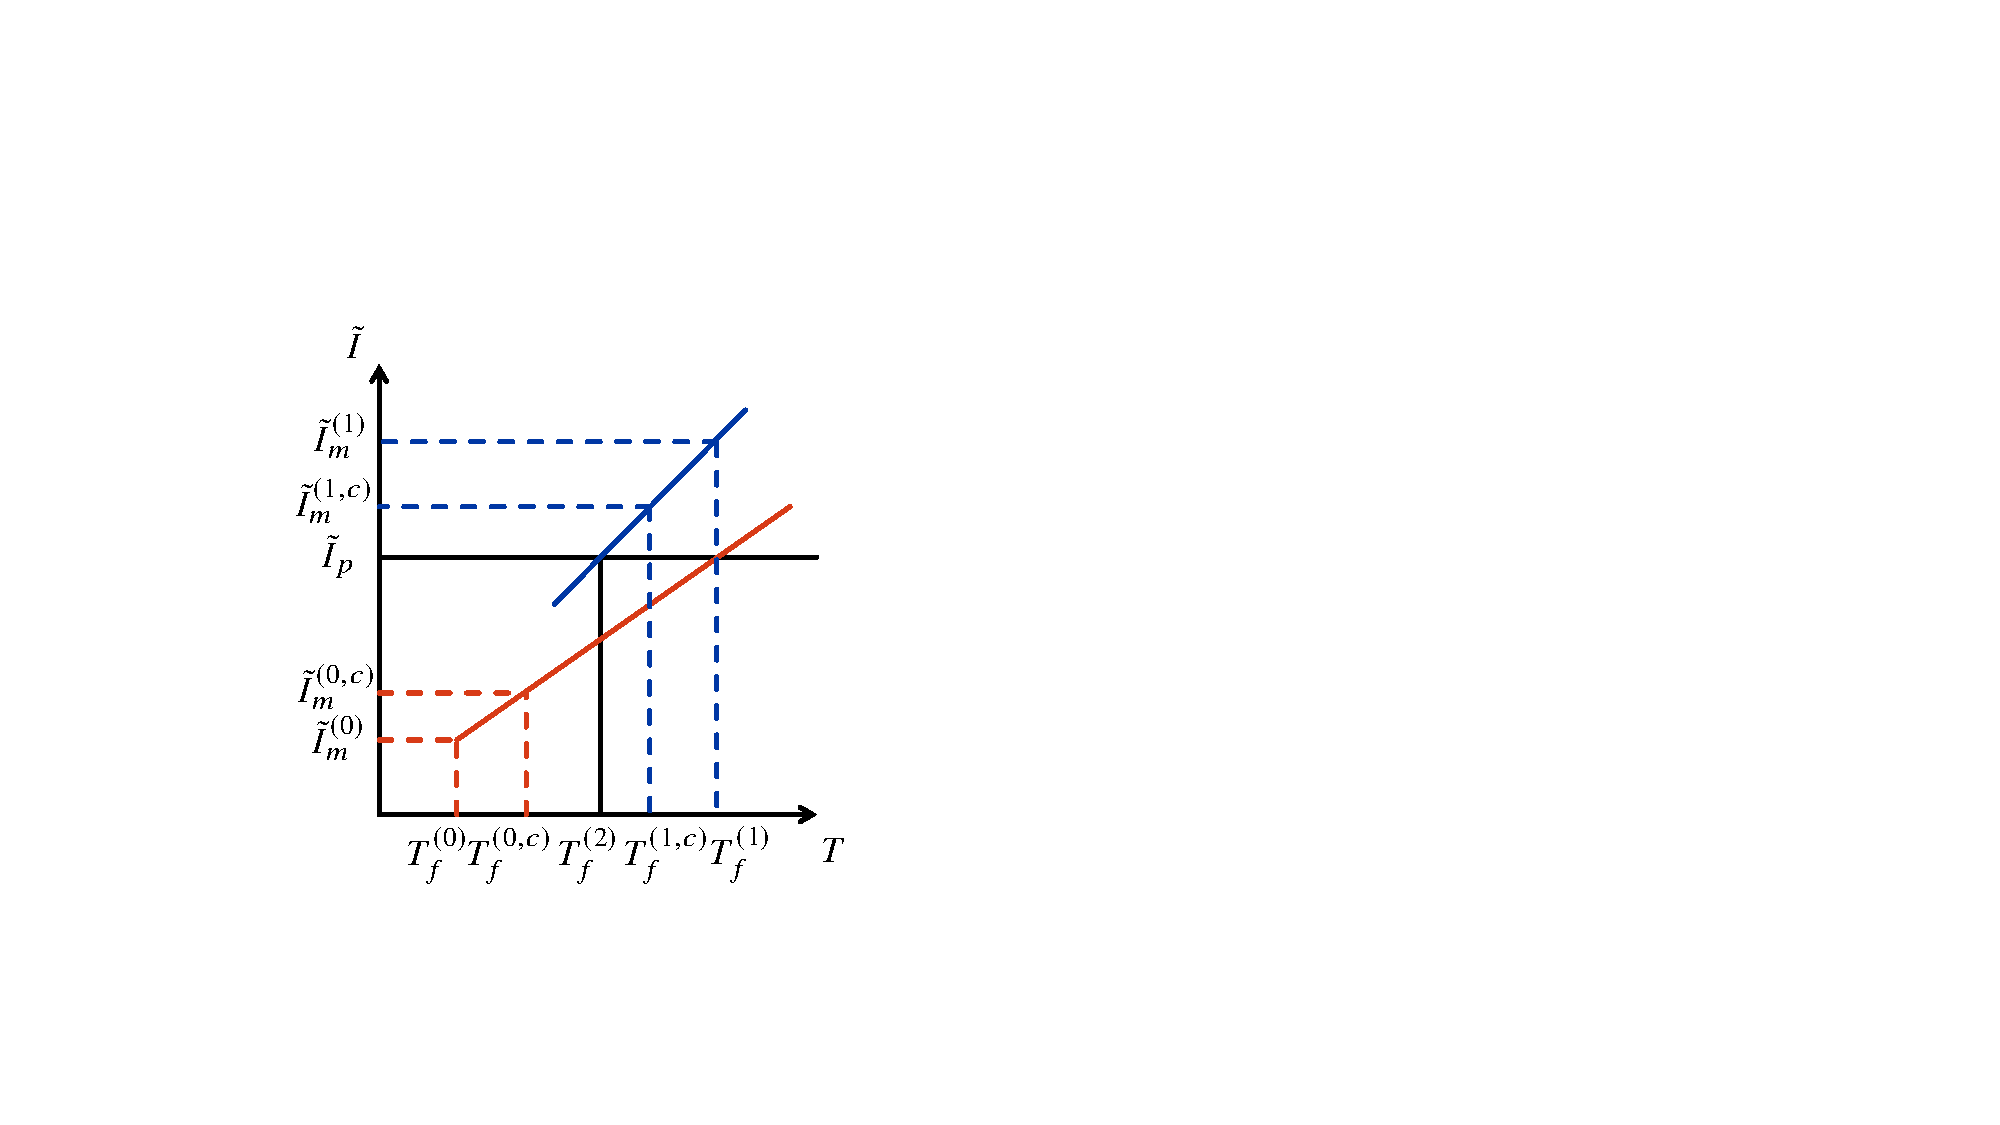
\includegraphics[width=0.8\linewidth]{pic/线性修正.pdf}
		\vspace*{0.8em}
		\caption{$T_\f$线性修正}
	\end{minipage}
	\begin{minipage}{0.45\linewidth}
		\centering
		\vspace*{0.7em}
		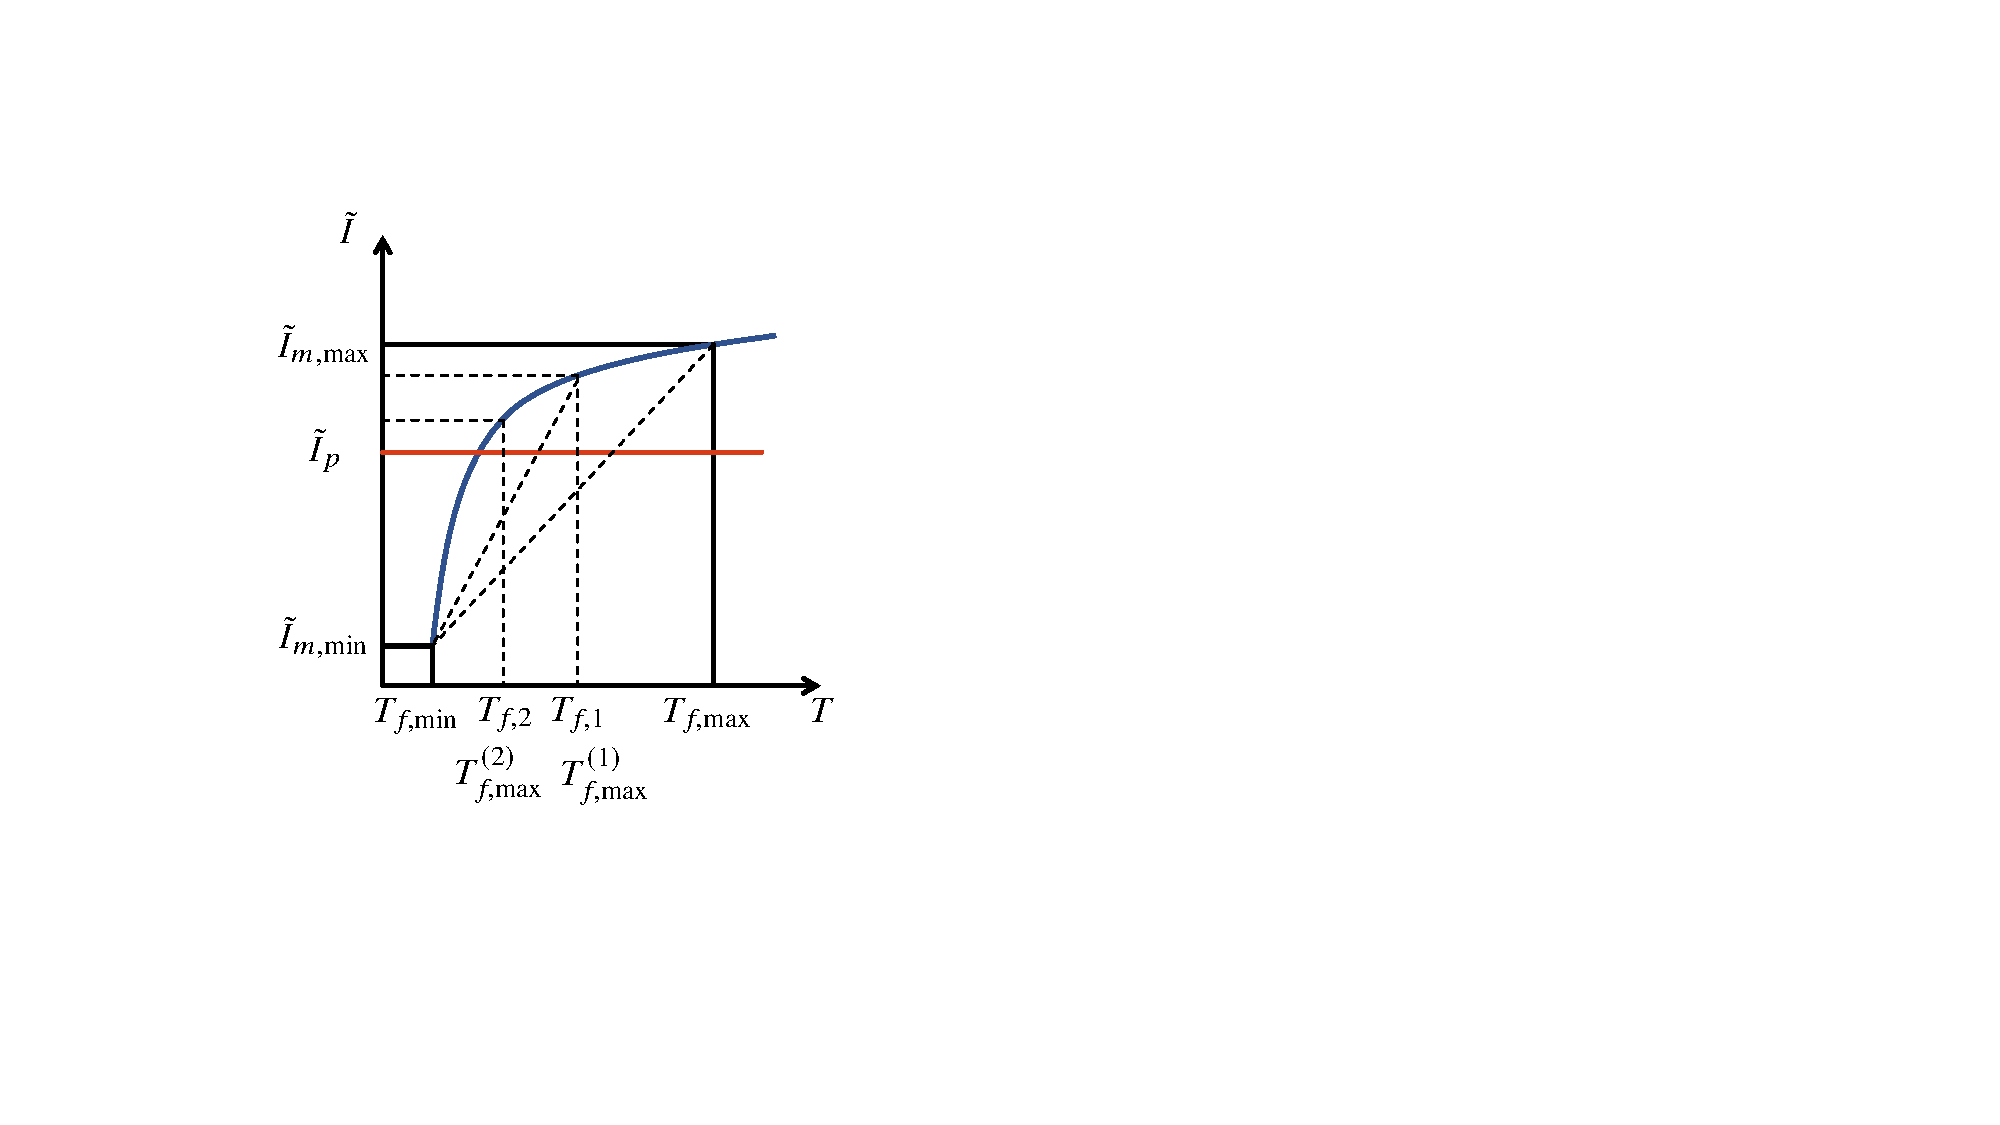
\includegraphics[width=0.85\linewidth]{pic/内插法修正.pdf}
		\vspace*{-0.8em}
		\caption{$T_\f$内插法修正}
	\end{minipage}
\end{figure}

	\item \textbf{内插法}\\
	\hspace*{2em}  预先设定的最小最大温度,可以取为常温和合理的极限温度\footnote[1]{\blue[双基推进剂的绝热燃烧温度在2000$\sim$3000K之间;复合推进剂燃烧温度可达到3000$\sim$4000K。]}。\\
	收敛标准
	\begin{equation}
		\left|\dfrac{T_{f,k}-T_{f,k-1}}{T_{f,k}}\right| \le \varepsilon_T \quad \mbox{或} \quad \left|T_{f,k} - T_{f, k - 1}\right| \le e_T
	\end{equation}
\end{enumerate}
\vspace*{0.5em}

\sssection[燃烧产物的热力学性质]
\begin{enumerate}[\hspace*{2em} (1) ]
	\item \textbf{凝相产物的质量百分数$\varepsilon$}
	\begin{equation}
		\varepsilon = \sum_{j = 1}^{L} \dfrac{m_j n_j}{1000}
	\end{equation}
	
	\item \textbf{气相产物的平均摩尔质量}
	\begin{equation}
		\overline{m} = 1000 \cdot \dfrac{1 - \varepsilon}{n_g}
	\end{equation}
	
	\item \textbf{气相产物的平均气体常数}
	\begin{equation}
		\overline{R} = \dfrac{R_0}{\overline{m}}
	\end{equation}

	\item \textbf{声速}
	\begin{itemize}
		\item 平衡时声速
		\begin{equation}
			a^2 = \left(\dfrac{\partial P}{\partial \rho}\right)_S = \dfrac{kR_0 T}{\overline{m}\left[1 + \left(\dfrac{\partial \ln \overline{m}}{\partial \ln p}\right)_T\right]}
		\end{equation}
		\item 组分冻结时
		\begin{equation}
			\left(\dfrac{\partial \ln \overline{m}}{\partial \ln p}\right)_T = 0 \quad \Rightarrow \quad a_\f = \sqrt{k\overline{R}T}
		\end{equation}
	\end{itemize}

	\item \textbf{比热与比热比}\\[0.5em]
	定压比热$c_p = \left(\dfrac{\partial \tilde{H}}{\partial T}\right)_p$,定容比热$c_v = \left(\dfrac{\partial \tilde{E}}{\partial T}\right)_v$.\vspace*{-0.5em}
	\begin{itemize}
		\item 定压比热
		\begin{equation}
			c_p = \dfrac{\partial }{\partial T} \left(\sum_{j = 1}^{N} H_j n_j\right)_p = \mathop{\sum_{j = 1}^{N} n_j \left(\dfrac{\partial H_j}{\partial T}\right)_p}_{\scriptsize \mbox{\blue[每种组分的焓值变化]}} + \mathop{\sum_{j = 1}^{N} H_j \left(\dfrac{\partial n_j}{\partial T}\right)_p}_{\scriptsize \mbox{\blue[组分变化引起的焓变]}}
		\end{equation}
	
		\item 平衡定压比热
		\begin{equation}
			c_p = \sum_{j = 1}^{N} n_j \left(\dfrac{\partial H_j}{\partial T}\right)_p\sum_{j = 1}^{N} H_j \left(\dfrac{\partial n_j}{\partial T}\right)_p =  \sum_{j = 1}^{N} n_j c_{pj} + \dfrac{1}{T}\left(\sum_{j = 1}^{N} n_j H_j D_{Tj}\right), \qquad D_j =\left(\dfrac{\partial \ln n_j}{\partial \ln T}\right)_p
		\end{equation}
	
		\item 冻结定压比热
		\begin{equation}
			c_{p,\f} =  \dfrac{\partial }{\partial T} \left(\sum_{j = 1}^{N} H_j n_j\right)_p = \sum_{j = 1}^{N} n_j \left(\dfrac{\partial H_j}{\partial T}\right)_p = \sum_{j = 1}^{N} n_j c_{pj}
		\end{equation}
	
		\item 定容比热
		\begin{equation}
			c_v = \left(\dfrac{\partial \tilde{E}}{\partial T}\right)_v = c_p - \dfrac{R_0\left[1 - \left(\dfrac{\partial \ln \overline{m}}{\partial \ln T}\right)_p \right]}{\overline{m}\left[1 + \left(\dfrac{\partial \ln \overline{m}}{\partial \ln p}\right)_T \right]}
		\end{equation}
	
		\item 冻结定容比热
		\begin{equation}
			c_{v,\f} = c_{p,\f} + \dfrac{R_0}{\overline{m}} = c_{p,\f} + \overline{R}
		\end{equation}
		
		\item 比热比
		\begin{equation}
			k = \dfrac{c_p}{c_v}
		\end{equation}
	
		\item 冻结比热比
		\begin{equation}
			k_\f = \dfrac{c_{p,\f}}{c_{v,\f}}
		\end{equation}
	\end{itemize}
\end{enumerate}
\vspace*{-0.5em}

\warn
[
	\hspace*{1.5em} 严格来说,平衡参数与冻结参数是有一定差别的,特别在燃气的成分随着温度或压强的改变而急剧变化的情况下,二者的差别更为明显。
	
	\hspace*{1.5em} 只有当燃气的成分不随温度和压强而改变(也即当燃气尚未离解,或者完全离解时),平衡参数与冻结参数才相一致。
]
\vspace*{0.5em}

\sssection[燃烧产物的熵]

化学物质的熵取决于它的分子结构和它所处的温度和压强。
\begin{equation}
	\tilde{S} = \sum_{j = 1}^N S_jn_j = \mathop{\sum_{j = 1}^{L} S_j n_j}_{\scriptsize \mbox{\blue[凝相组分的熵]}} + \mathop{\sum_{j = L + 1}^N S_j n_j}_{\scriptsize \mbox{\blue[气相组分的熵]}} 
\end{equation}
其中,$\tilde{S}$为1$\,$kg燃烧产物的熵,$n_j$为各组分的摩尔数。

对气相组分
\begin{equation}
	S_j = S_j^0 - R_0 \ln p_j \qquad (j = L + 1, L + 2, \cdots , N)
\end{equation}

对凝相组分
\begin{equation}
	S_j = S_j^0 \qquad (j = 1,2, \cdots , L)
\end{equation}
结合可得,
\begin{equation}
	\tilde{S} = \sum_{j  = 1}^{N} S_j^0 n_j - R_0 \left[n_g \ln p + \sum_{j = L +1}^{N} n_j \ln \left(\dfrac{n_j}{n_g}\right)\right]
\end{equation}
其中,$S_j^0$为1$\,$mol$j$组分在一个物理大气压以及绝热温度$T_\f$条件下的熵;$p_j$为$j$组分的分压,单位均取atm.
\vspace*{1em}
\clearpage

\sssection[燃烧产物的输运性质]

\defination[输运过程]
{
	\dy[输运过程]{SYGC}\quad 导致系统从不平衡到平衡的过程。
	{
		\begin{equation*}
			\begin{cases}
				\, \mbox{\dy[动量输运过程]{DLSYGC}:是系统内宏观的相对运动逐渐消失,最终到达系统内速度处处相等。} \rightarrow \mbox{\dy[粘性系数]{NXXS}}\, \mu \\
				\, \mbox{\dy[热量输运过程]{RLSYFC}:使系统内各处的温差逐渐消失,最终达到各处的温度相等。}\rightarrow \mbox{\dy[热传导系数]{RCDXS}}\, \lambda \\
				\, \mbox{\dy[质量输运过程]{ZLSYGC}:使系统内各处的浓度逐渐达到一直而处于均匀状态。}\rightarrow\mbox{\dy[扩散系数]{KSXS}}\, D
			\end{cases}
		\end{equation*}
		\vspace*{-0.5em}
	}
}
\vspace*{-1em}

\begin{enumerate}[\hspace*{1.5em} (1) ]
	\item \textbf{粘性系数$\mu$的计算}
	\begin{equation}
		\begin{cases}
			\, \mu = \dfrac{1}{3}n \overline{v}m_0l\\[0.5em]
			\, l = \dfrac{1}{\sqrt{2} \pi d^2 n}\\[1em]
			\, \overline{v} = \sqrt{\dfrac{8k_0T}{\pi m_0}}
		\end{cases}
		\quad \Rightarrow \quad \mu = \dfrac{2}{3}\dfrac{1}{\pi^{\textstyle \frac{3}{2}}}\dfrac{\sqrt{m_0k_0T}}{d^2}
	\end{equation}
	其中,\vspace*{-1em}
	\begin{itemize}
		\item $\overline{v}$ \quad 气体分子的平均速度(算术平均值)\vspace*{-0.5em}
		\item $n$ \quad 容器内气体分子数\vspace*{-0.5em}
		\item $d$ \quad 气体分子的平均直径\vspace*{-0.5em}
		\item $m_0$ \quad 单个气体的平均质量\vspace*{-0.5em}
	\end{itemize}
	实际常采用\dy[Sutherland公式]{SUTHERLANDGS}
	\begin{equation}
		\mu_1 = u_0 \left(\dfrac{T}{273}\right)^{1.5} \cdot \dfrac{273 + T_0}{T + T_0}
	\end{equation}
	
	\item \textbf{能量输运过程中热传导系数$\lambda$的计算}\vspace*{-1em}
	\begin{itemize}
		\item \dy[傅立叶定律]{FLYDL}
		\begin{equation}
			q = - \lambda \dfrac{\d T}{\d y}
		\end{equation}
		\item 单种气体
		\begin{equation}
			\lambda_i = \dfrac{R_0\mu_i}{m_i}\left(0.45 + 1.32 \dfrac{c_{pi}}{R_0}\right)
		\end{equation}
		\item 混合气体
		\begin{equation}
			\lambda = \sum_{i = L +1}^{N} \lambda_i \left[ {\displaystyle 1 + 1.065 \sum_{j =L+1, j \neq i}^{N} \phi_{ij}\dfrac{Z_j}{Z_i}}\right]^{-1}
		\end{equation}
	\end{itemize}
\end{enumerate}

\subsection{燃烧室热力计算总结}
	燃烧室热力计算任务的本质:在给定推进剂组分和总焓、平衡压强的条件下, 计算推进剂的绝热燃烧温度、燃烧产物组分及其各种特性参数。\red[三大核心输入条件:推进剂组分、总焓和平衡压强],\blue[两项核心任务:计算平衡组分、根据平衡组分计算绝热燃烧温度]。由于数学模型的复杂性,无法直接联立求解。只能采用迭代法:
	\begin{equation*}
		\mbox{假定燃烧温度}\, \longrightarrow \, \mbox{平衡计算} \, \longrightarrow \, \mbox{求解\&修正温度}\, \longrightarrow \, \mbox{平衡计算} \, \xrightarrow{\scriptsize \,\,\,\mbox{结果收敛}\,\,\,} \, \mbox{实际燃烧温度,平衡组分,特性参数}
	\end{equation*}
总体概括如图\ref{化学平衡热力计算总体图}所示.
\begin{figure}[!htb]
	\centering
	\begin{tikzpicture}
		\node (B)  [inner sep = 5pt, draw ]{\red[化学平衡热力计算]};
		\node (A) [inner sep = 5pt, draw, node distance = 5.3cm, left of = B]{\blue[推进剂组分\quad 总焓 \quad 平衡压强]};
		\node (C)[inner sep = 5pt,  draw, node distance = 6.1cm, right of = B]{\blue[绝热燃烧温度\quad 平衡组分 \quad 产物特性参数]};
		
		\draw[arrows={-Stealth}] (A) -- (B)node[midway, above = 0cm]{\scriptsize 假定温度};
		\draw[arrows={-Stealth}] (B) -- (C)node[midway, above = 0cm]{\scriptsize 迭代修正};
		
	\end{tikzpicture}
	\caption{化学平衡热力计算的总体过程图}
	\label{化学平衡热力计算总体图}
\end{figure}

\section{喷管流动过程的热力计算}
\subsection{喷管热力计算的任务及已知条件}
\sssection[基本任务]
\vspace*{-1em}

\begin{enumerate}[\hspace*{1.5em} (1) ]
	\item  计算喷管任一截面上(尤其是出口截面上)燃烧产物的组分、温度及热力学参数,即$n_{ji},P_i,T_i,H_i,S_i$等\vspace*{-0.5em}
	\item 计算喷管指定界面上(尤其是出口截面上)燃烧产物的流速$v$和发动机理论比冲$I_s$
\end{enumerate}
\vspace*{0.5em}

\sssection[已知条件]
\vspace*{-1em}

\begin{enumerate}[\hspace*{1.5em} (1) ]
	\item  燃烧室热力计算的结果,也即喷管入
口截面上燃烧产物的热力学参数(如$P_{0\c},T_{0\f},k,S_{0\c}$等)及产物组分等摩尔数$n_j$等\vspace*{-0.5em}
	\item 表示喷管计算截面的参数(如给定喷管出口参数$P_\e , \text{Ma}$等)\blfootnote{$\,^*$\dy[不可逆现象]{BKNXX}:摩擦、传热及其它的不平衡现象}
\end{enumerate}

\subsection{喷管热力计算模型}
\sssection[热力计算模型]
\begin{figure}[!htb]
	\centering
	\begin{tikzpicture}
		\node (A) [draw, inner sep = 5pt]{喷管流动过程分析};
		\node (A1) [draw, inner sep = 5pt, right of = A, yshift = 2cm, node distance = 8.5cm]{燃烧产物等压强下降($p \downarrow$),温度下降($T\downarrow$),产物的流速增大$V \uparrow$};
		\node (A2) [draw, inner sep = 5pt, right of = A, yshift = 1cm, node distance =8.7cm]{$P \downarrow, T\downarrow\, \rightarrow\,$复合反应$\,\rightarrow\,$放热且产物组分改变$\,\rightarrow\,$$A+B \ce{<=>} AB + Q$};
		\node (A3)  [draw, inner sep = 5pt, right of = A, yshift = 0cm, node distance =5.68cm]{流动过程是化学非平衡过程};
		\node (A4)  [draw, inner sep = 5pt, right of = A, yshift = -1cm, node distance =5cm]{存在能量平衡问题};
		\node (A5)  [draw, inner sep = 5pt, right of = A, yshift = -2cm, node distance =4.81cm]{存在相平衡问题};
		
		\node (B) [draw, inner sep =5pt, below of = A, node distance = 4cm]{简化假设};
		\node (B1) [draw, inner sep = 5pt, right of = B, yshift = 0.5cm, node distance = 6.05cm]{燃烧产物是组分均一的完全气体};
		\node (B2) [draw, inner sep = 5pt, right of = B, yshift = -0.5cm, node distance = 7.95cm]{流动过程是一个\blue[不存在任何不可逆现象]$\,^*$的理想流动过程};
		
		\node (C) [draw, inner sep =5 pt, below of = B, node distance = 3.cm]{热力计算理论模型};
		\node (C1) [draw, inner sep = 5pt, right of = C, node distance = 4.65cm]{等熵流动模型};
		\node (C2) [draw, inner sep = 5pt, right of = C1, node distance = 3.2cm]{$S = \text{Const.}$};
		\node (C31) [draw, inner sep = 5pt, right of = C2, yshift = 1cm, node distance = 3.4cm]{平衡流动模型};
		\node (C32) [draw, inner sep = 5pt, right of = C2, yshift = 0cm, node distance = 4.3cm]{化学组分冻结的流动模型};
		\node (C33) [draw, inner sep = 5pt, right of = C2, yshift = -1cm, node distance = 4.65cm]{化学组分突然冻结的流动模型};
		
		\draw[arrows={-Stealth}] (A) -- (B);
		\draw[arrows={-Stealth}] (B) -- (C);
		\draw (A)  -- +(2.4cm,0cm) -- +(2.4cm, 2cm) -- (A1);
		\draw (A)  -- +(2.4cm,0cm) -- +(2.4cm, 1cm) -- (A2);
		\draw (A)  -- (A3);
		\draw (A)  -- +(2.4cm,0cm) -- +(2.4cm, -1cm) -- (A4);
		\draw (A)  -- +(2.4cm,0cm) -- +(2.4cm, -2cm) -- (A5);
		\draw (B)  -- + (2.43cm,0cm) -- +(2.43cm,0.5cm) -- (B1);
		\draw (B)  -- + (2.43cm,0cm) -- +(2.43cm,-0.5cm) -- (B2);
		\draw (C)  -- (C1) -- (C2);
		\draw (C2) --+ (1.5cm, 0cm) --+ (1.5cm, 1cm) -- (C31);
		\draw (C2) -- (C32);
		\draw (C2) --+ (1.5cm, 0cm) --+ (1.5cm, -1cm) -- (C33);
	\end{tikzpicture}
\end{figure}
\clearpage

由上面的模型,可以得到喷管的热力计算方程。
\vspace*{0.5em}

\sssection[等熵方程]

由喷管任一截面上燃烧产物的熵值$ = $喷管入口截面上燃烧产物的熵值,可以得到
\begin{equation}
	S(p,T) = S_{0\c}
\end{equation}
而
\begin{equation}
	S = \sum_{j = 1}^{N}S_j^0n_j - R_0 \sum_{j = L + 1}^{N} n_j \ln \left(\dfrac{n_j}{n_g}\right) - R_0 n_g \ln P
\end{equation}
其中,$S_j^0$是1$\,$mol$j$组分在一个大气压及燃烧温度$T_\f$条件下的熵。记为方程
\begin{equation}
	\varphi_1 = S(P, T) - S_{0\c} = 0
\end{equation}

\sssection[表示喷管计算截面的方程]
\vspace*{-0.5em}
\begin{itemize}
	\item 给定喷管计算截面上的压强$P^{(\delta)}$:$P = P^{)\delta} = \text{Const.}$,对于完全膨胀的截面有$P_\e = P_\a$\vspace*{-0.5em}
	\item 给定喷管压强比$\varepsilon_p^{(\delta )}$:$P - \varepsilon_p^{(\delta)} P_{0\c} = 0\, \Rightarrow \, \varepsilon_p = \dfrac{P}{P_{0\c}}$ \vspace*{-0.5em}
	\item 给定喷管面积比$\varepsilon_A^{(\delta)}$:$\dfrac{\rho_t  u_t }{\rho u} =\varepsilon_A^{(\delta)}$\vspace*{-0.5em}
	\item 给定喷管计算截面的马赫数$M^{(\delta)}$:$\dfrac{\sqrt{2\big(I_{m,0\c} - I_m\big)}}{a} - M^{(\delta)} = 0$\vspace*{-0.5em}
	\item 给定喷管计算截面的温度$T^{(\delta)}$:$T = T^{(\delta)} = \text{Const.}$
\end{itemize}
引入函数$\varphi_2$,得
\begin{equation}
	\varphi_2(P, T) = 0
\end{equation}

\sssection[喷管热力计算方程]
\begin{equation*}
	\begin{cases}
		\mbox{等熵方程} & \varphi_1 = \tilde{S}(P, T) - \tilde{S}_{0\c} = 0\\
		\mbox{喷管计算方程} & \varphi_2(p, T) = 0\\
		\mbox{质量守恒和化学平衡方程} & \mbox{计算}\, n_j
	\end{cases}
\end{equation*}

\warn[\hspace*{1.5em} 喷管流动过程存在{\red[能量转换]}(内能$\, \to \,$动能),燃烧产物的{\red[总焓不守恒、能量仍守恒]}。]

现在只知道热力计算三大核心条件之一:推进剂组分,而其他两个量:总焓和平衡压强仍未知,下面分情况求解。


\subsection{典型的喷管流动计算}

\sssection[平衡膨胀到给定马赫数$M$(包括喷管喉部截面)]
\begin{equation*}
	\red[\mbox{核心问题:确定总焓} \,I\, \mbox{和压强}\, p]\, 
	\begin{cases}
		\, \mbox{核心条件:等熵、平衡、给定}\, M \\
		\, \mbox{冻结流:等熵流动公式:}(P_{0c} , T_{0c}, M) \, \to \, (p, T)\\
		\, \mbox{平衡流:}\, p \, \mbox{变化} \,\to \, \mbox{平衡状态变:}(n_j, T)\, \to \, (v, M, \cdots)
	\end{cases}
\end{equation*}
\blue[注意:能量转换$\, \to \,$动能$\, \to \,$ 总焓不守恒,能量仍守恒]
\clearpage

\begin{figure}[!htb]
	\centering
	\begin{tikzpicture}
		\node (A) [draw, inner sep = 5pt]{\makecell[c]{按\blue[冻结流]\\[-0.3em]预估气流参数}};
		\node (B) [draw, inner sep = 5pt, right of = A, node distance = 6.3cm]{计算指定截面的总焓};
		\node (C) [draw, inner sep = 5pt, right of = B, node distance = 7.7cm]{化学平衡计算};
		\node (D) [draw, inner sep = 5pt, below of = B, xshift = 4cm, node distance = 2cm]{依据等熵条件\textbf{修正压强}};
		
		\draw[arrows={-Stealth}] (A) -- (B)node[midway, above = 0cm]{$p, T ,v$}node[midway, below = 0cm]{$\displaystyle I_m = I_{m,0\c} - \dfrac{1}{2}\left(aM\right)^2$};
		\draw[arrows={-Stealth}] (B) -- (C)node[midway, above = 0cm]{\scriptsize \blue[组分,总焓,压强]};
		\draw[arrows={-Stealth}] (C) -- +(0cm, -2cm) -- (D)node[midway, above = 0cm]{\scriptsize \blue[温度,组分]}node[midway, below = 0cm]{\scriptsize \blue[特性]};
		\draw[arrows={-Stealth}] (D) -- +(-4cm , 0cm)node[midway, above = 0cm]{$P$} -- (B)node[very near start, left = 0cm]{$\displaystyle S = \sum_{j = 1}^{N}S_j^0 n_j - R_0 \sum_{j = L + 1}^{N} n_j \ln \left(\dfrac{n_j}{n_g}\right) - R_0 n_g \ln P$};
	\end{tikzpicture}
	\caption{平衡膨胀到给定马赫数求解流程图}
	\label{平衡膨胀马赫数}
\end{figure}

\sssection[燃烧产物膨胀到给定压强$P_e$]

最典型、最常遇到的情况:在设计状态下,计算喷管出口截面上的燃气参数。在设计状态下有:
\begin{equation*}
	P_\e = P_\a
	\, 
	\begin{cases}
		\, \mbox{\red[冻结膨胀]} \, \longrightarrow \, \mbox{产物组分不变,采用等熵流计算方法即可}\\
		\, \mbox{\red[平衡膨胀]} \, \longrightarrow \, \mbox{产物组分改变,当地状态下热力平衡}
	\end{cases}
\end{equation*}		

\begin{equation*}
	\red[\mbox{核心问题:确定总焓} \,I\, \mbox{和压强}\, p]\, 
	\begin{cases}
		\, \mbox{核心条件:等熵、平衡、给定}\, P_e \\
		\, \mbox{冻结流:等熵流动公式:}(p_\t , T_\t, p_\e) \, \to \, (T_\e, M_\e)\\
		\, \mbox{平衡流:}\, p \, \mbox{变化} \,\to\, \mbox{平衡状态变:}(n_j, T_\e)\, \to \, (v_\e, M_\e, \cdots)
	\end{cases}
\end{equation*}
\blue[注意:能量转换$\, \to \,$动能$\, \to \,$ 总焓不守恒,能量仍守恒]。
\begin{figure}[!htb]
	\centering
	\begin{tikzpicture}
		\node (A) [draw, inner sep = 5pt]{\makecell[c]{按\blue[冻结流]\\[-0.3em]预估气流参数}};
		\node (B) [draw, inner sep = 5pt, right of = A, node distance = 6.3cm]{计算指定截面的总焓};
		\node (C) [draw, inner sep = 5pt, right of = B, node distance = 7.7cm]{化学平衡计算};
		\node (D) [draw, inner sep = 5pt, below of = B, xshift = 4cm, node distance = 2cm]{依据等熵条件\textbf{修正温度}};
		
		\draw[arrows={-Stealth}] (A) -- (B)node[midway, above = 0cm]{$T_\e ,v$}node[midway, below = 0cm]{$\displaystyle I_m = I_{m,0\c} - \dfrac{1}{2}v^2$};
		\draw[arrows={-Stealth}] (B) -- (C)node[midway, above = 0cm]{\scriptsize \blue[组分,总焓,压强]};
		\draw[arrows={-Stealth}] (C) -- +(0cm, -2cm) -- (D)node[midway, above = 0cm]{\scriptsize \blue[温度,组分]}node[midway, below = 0cm]{\scriptsize \blue[特性]};
		\draw[arrows={-Stealth}] (D) -- +(-4cm , 0cm)node[midway, above = 0cm]{$T_\e$} -- (B)node[very near start, left = 0cm]{$\displaystyle S = \sum_{j = 1}^{N}S_j^0 n_j - R_0 \sum_{j = L + 1}^{N} n_j \ln \left(\dfrac{n_j}{n_g}\right) - R_0 n_g \ln P$};
	\end{tikzpicture}
	\caption{平衡膨胀到给定压强求解流程图}
	\label{平衡膨胀压强}
\end{figure}
\vspace*{-0.5em}

注:等熵过程公式为
\begin{equation}
	T'_\e = T_\c \left(\dfrac{p_\e}{p_\c}\right)^{\textstyle \frac{k-1}{k}}
	\label{等熵流动}
\end{equation}

\section{发动机理论性能参数计算}

\sssection[基本假设]\vspace*{-1em}
\begin{enumerate}[\hspace*{1.5em} (1) ]
	\item 推进剂燃烧完全,产物在流动过程中处于平衡冻结状态\vspace*{-0.5em}
	\item 燃烧产物中气相产物为完全气体\vspace*{-0.5em}
	\item 喷管内流动是一维的\vspace*{-0.5em}
	\item 燃烧过程是绝热的,喷管的流动过程是定常的、而且是等熵的
\end{enumerate}

\sssection[两种方法计算理论性能]\vspace*{-1em}
\begin{enumerate}[\hspace*{1.5em} (1) ]
	\item 在热力计算结果的基础上进行计算(本章)\vspace*{-0.5em}
	\item 利用气体流动力学中的气动关系式及平均等熵指数进行计算(第二章)
\end{enumerate}

\subsection{发动机理论性能参数计算}

\sssection[利用热力计算结果计算发动机理论性能]\vspace*{-1em}
\begin{enumerate}[\hspace*{1.5em} (1) ]
	\item \textbf{喷气速度$u_e$}
	\begin{equation}
		\begin{cases}
			\, \tilde{I}_{m,0\c} + \dfrac{u_{0\c}^2}{2} = \tilde{I}_{m,\e} + \dfrac{u_\e^2}{2} \\
			\, u_{0\c}\le u_\e
		\end{cases}
		\quad \Rightarrow \quad 
		u_\e = \sqrt{2 (\tilde{I}_{m,0\c} - \tilde{I}_{m,\e})} 
	\end{equation}
	其中,$\tilde{I}_{m,0\c}$是喷管入口截面上燃烧产物的总焓,$\tilde{I}_{m,\e}$是喷管出口截面上燃烧产物的总焓。对于化学组分冻结的喷管流动,化学能不变化,则
	\begin{equation}
		u_\e = \sqrt{2\big(H_{m,0\c} - H_{m,\c}\big)}
	\end{equation}

	\item \textbf{理论比冲$I_s$}
	\begin{equation}
		I_s = u_\e + \dfrac{A_\e}{\dot{m}}(p_\e - p_\a) \quad \Rightarrow \quad 
		\begin{cases}
			\, \mbox{真空比冲} & I_{s,v} = u_\e + \dfrac{A_\e}{\dot{m}}p_\e\\
			\, \mbox{设计状态比冲} & I_s = u_\e (p_e = p_\a)
		\end{cases}
	\end{equation}

	\item \textbf{理论特征速度$c^*$}
	\begin{equation}
			\begin{cases}
				c^* = \dfrac{P_{0\c A_\t}}{\dot{m}}\\
				\dot{m} = \rho_\t A_\t u_\t\\
				p_\t = \rho_\t \overline{R}_\t T_\t
			\end{cases}
			\quad \Rightarrow \quad c^* = \dfrac{P_{0\c}A_\t}{\dot{m}} = \dfrac{P_{0\c}A_\t}{\rho_\t A_\t u_\t} = \dfrac{p_{0\c}}{p_\t} \cdot \dfrac{R_0}{\overline{M}_\t}\cdot\dfrac{T_\t}{u_\t}
	\end{equation}

	\item \textbf{理论推力系数$C_F$}
	\begin{equation}
		C_F = \dfrac{I_s}{c^*} = 
		\begin{cases}
			\, \mbox{真空中的理论推力系数} & C_{F,V} = \dfrac{I_{s,V}}{c^*}\\
			\, \mbox{设计状态的理论推力系数} & C_F = \dfrac{u_\e}{c^*}
		\end{cases}
	\end{equation}
\end{enumerate}

\sssection[气动关系式及平均等熵指数计算发动机理论性能]

	纯气相燃烧产物在喷管中流动被认为是等熵的,由等熵过程伯努利方程
	\begin{equation}
		\dfrac{k}{k - 1} \dfrac{p}{\rho} + \dfrac{u^2}{2} = \mathrm{C}
	\end{equation}
又由等熵关系式
	\begin{equation}
		\dfrac{p}{\rho^k} = \mathrm{C}
	\end{equation}
结合气体状态方程可以得到排气速度
	\begin{equation}
		u_\e = \sqrt{2 \dfrac{k}{k - 1} R_\c T_\c \left[1 - \left(\dfrac{p_\e}{p_\c}\right)^{\textstyle \frac{k-1}{k}}\right]}
	\end{equation}
利用喉部速度为声速及响应热力关系式,可推导得质量流量
\begin{equation}
	\dot{m} = \varGamma \dfrac{A_\t p_\c}{\sqrt{R_\c T_\c}}
\end{equation}
可以得到比冲与真空比冲
\begin{equation}
	I_s = u_\e + \dfrac{A_\e}{\dot{m}}(p_\e - p_\a) \qquad I_{s,V} = u_\e + \dfrac{A_\e}{\dot{m}}p_\e
\end{equation}
\vspace*{0.3em}

\subsection{发动机理论性能参数的影响因素}

\sssection[膨胀压强比和燃烧室压强对发动机性能影响]
\begin{equation*}
	u_\e = \sqrt{2 \dfrac{k}{k - 1} R_\c T_\c \left[1 - \left(\dfrac{p_\e}{p_\c}\right)^{\textstyle \frac{k-1}{k}}\right]}
\end{equation*}
	推进剂确定,压强膨胀比也确定,当燃烧室压强增加,燃烧产物的离解浓度减小。对性能影响先增加,而后逐渐趋于平缓。
	
	当推进剂确定燃烧室压强也确定,膨胀比对发动机性能有提高作用。\textbf{但是需要同时考虑发动机强度、结构尺寸和质量等。}
\vspace*{0.8em}

\sssection[喷管平衡/冻结流动模型的影响]

燃烧室高温高压状态下,化学反应程度剧烈,解离反应较多。喷管中气流温度和压强下降较大(压强可降2个量级),容易发生复合反应,释放热量。
\vspace*{0.8em}

\sssection[喷管中的实际流动过程与损失]\vspace*{-1em}
\begin{enumerate}[\hspace*{1.5em} (1) ]
	\item 实际流动不是纯气相的:\dy[二相损失$\xi_p$]{EXSS}\vspace*{-0.5em}
	\item 燃气与喷管壁面间有传热的摩擦:\dy[散热损失$\xi_q$]{SRSS}和\dy[摩擦损失$\xi_f$]{MCSS}\vspace*{-0.5em}
	\item 实际流动是二维或三维的:\dy[非轴向损失$\xi_a$]{FZXSS}\vspace*{-0.5em}
	\item 实际流动是化学不平衡流动:\dy[化学不平衡损失$\xi_n$]{HXBPHSS}\vspace*{-0.5em}
	\item 高温气体有可能是喷管烧蚀:\dy[喷管烧蚀损失$\xi_e$]{PGSSSS}
\end{enumerate}
可以得到\dy[冲量系数$\xi_N$]{CLXS}
\begin{equation}
	\xi_N = \xi_a \xi_n \xi_p \xi_q \xi_f \xi_e
\end{equation}

\subsection{发动机性能热力计算全过程}
见下页图\ref{发动机总结}所示.
\clearpage

\begin{figure}[!htb]
	\centering
	\begin{tikzpicture}
		\node (A) [draw, inner sep = 5pt]{开始};
		\node (B) [draw, inner sep = 5pt, below of = A, node distance = 2cm]{输入初始量};
		\node (B1) [draw, inner sep = 4pt, right of = B, node distance = 5.52cm, yshift = 1.6cm]{\small 假定化学式};
		\node (B2) [draw, inner sep = 4pt, right of = B, node distance = 5.06cm, yshift = 0.8cm]{\small 总焓};
		\node (B3) [draw, inner sep = 4pt, right of = B, node distance = 5.35cm, yshift = 0cm]{\small 初始温度};
		\node (B4) [draw, inner sep = 4pt, right of = B, node distance = 5.83cm, yshift = -0.8cm]{\small 燃烧室工作压强};
		\node (B5) [draw, inner sep = 4pt, right of = B, node distance = 6.0cm, yshift = -1.6cm]{\small 喷管出口截面压强};
		\node (C) [draw, inner sep = 5pt, below of = B, node distance = 1.3cm]{选定燃烧产物组分的种类};
		\node (D) [draw, inner sep = 5pt, below of = C, node distance = 1.3cm]{计算燃烧产物平衡组分的摩尔数,焓和熵};
		\node (E) [draw, inner sep = 5pt, below of = D, node distance = 1.3cm]{计算燃烧产物的绝热燃烧温度};
		\node (F) [draw, inner sep = 5pt, below of = E, node distance = 1.3cm]{计算给定压强和燃烧温度下产物平衡组分的摩尔数,焓和熵};
		\node (G) [draw, inner sep = 5pt, below of = F, node distance = 1.3cm]{计算燃烧产物的热力学特征参数};
		\node (G1) [inner sep =3pt, left of = C, node distance = 7cm, yshift = -2.6cm]{燃烧室热力计算};
		\node[diamond] (H) [draw, shape aspect = 4, inner sep = 3pt, below of = G, node distance = 1.5cm]{喷管流动过程};
		\node (I1) [draw, inner sep = 2pt, left of = H, node distance = 5.5cm]{\makecell[c]{选取喷管中的\\[-0.4em]平均等熵指数$k$}};
		\node (J1) [draw, inner sep = 5pt, below of = I1, node distance = 1.7cm]{选取试算温度$T_{\e1}<T_\e<T'_{\e2}$};
		\node (K1) [draw, inner sep = 5pt, below of = J1, node distance = 1.3cm]{计算燃烧产物的总焓和熵};
		\node (L1) [draw, inner sep = 5pt, below of = K1, node distance = 1.3cm]{计算燃烧产物在出口截面上的温度$T_\e$};
		\node (M1) [draw, inner sep = 5pt, below of = L1, node distance = 1.3cm]{确定出口截面产物的总焓};
		
		\node (I2) [draw, inner sep = 2pt, right of = H, node distance = 5cm]{\makecell[c]{选取喷管中的\\[-0.4em]平均等熵指数$k$}};
		\node (J2) [draw, inner sep = 5pt, below of = H, xshift = 1.5cm, node distance = 1.7cm]{选取试算温度$T_{\e1}<T_\e<T'_{\e2}$};
		\node (K2) [draw, inner sep = 5pt, below of = J2, node distance = 1.3cm]{产物平衡组分的摩尔数};
		\node (L2) [draw, inner sep = 5pt, below of = K2, node distance = 1.3cm]{计算燃烧产物燃烧产物的总焓和熵};
		\node (M2) [draw, inner sep = 5pt, below of = L2, node distance = 1.3cm]{计算燃烧产物在出口截面熵的温度$T_\e$};
		\node (O2) [draw, inner sep = 5pt, below of = M2, node distance = 1.3cm]{计算出口截面产物总焓及平衡组分的摩尔数};
		
		\node (P) [draw, inner sep = 5pt, below of = M1, node distance = 3.8cm]{计算热力学参数};
		\node (P1) [draw, inner sep = 4pt, right of = P, node distance = 7.7cm, yshift = 1.2cm]{\small 气相组分:摩尔总数,平均分子量,平均气体常数};
		\node (P2) [draw, inner sep = 4pt, right of = P, node distance = 5.935cm, yshift = 0.4cm]{\small 凝相组分:质量百分数};
		\node (P3) [draw, inner sep = 4pt, right of = P, node distance = 6.43cm, yshift = -0.4cm]{\small 整个燃烧产物的平均气体常数};
		\node (P4) [draw, inner sep = 4pt, right of = P, node distance = 5.765cm, yshift = -1.2cm]{\small 喷管平均等熵指数$\overline{k}$};
		\node (Q) [draw, inner sep = 5pt, below of = P, node distance = 1.5cm]{计算出口截面上燃烧产物的温度$T'_\e$};
		\node[diamond] (R) [draw, shape aspect = 5, inner sep = 3pt, below of = H, node distance = 12.9cm]{$T_{\e1} < T'_\e < T_{\e 2}?$};
		\node (R1) [draw, inner sep = 5pt, left of = R, node distance = 5cm]{$k = \overline{k}$};
		\node (R2) [draw, inner sep = 5pt, right of = R, node distance = 4.5cm]{$k = \overline{k}$};
		\node (S) [draw, below of = R, inner sep = 5pt, node distance = 1.6cm]{计算发动机理论比冲};
		\node (T) [draw, below of = R1, inner sep = 5pt, node distance = 1.6cm]{停止};
		\node (U)[below of = I2, inner sep = 1pt, node distance = 7.25cm, xshift = 2.2cm]{\makecell[c]{喷管流动\\[-0.5em]热力计算}};
		
		\draw[arrows={-Stealth}] (A) -- (B);
		\draw[arrows={-Stealth}] (B) -- (C)node[midway, left = 0cm]{\scriptsize 根据假定化学式};
		\draw[arrows={-Stealth}] (C) -- (D)node[midway, left = 0cm]{\scriptsize 指定燃烧室工作压强及温度}node[midway, right = 0cm]{\scriptsize 利用\blue[吉布斯自由能法]};
		\draw[arrows={-Stealth}] (D) -- (E);
		\draw[arrows={-Stealth}] (E) -- (F);
		\draw[arrows={-Stealth}] (F) -- (G);
		\draw[arrows={-Stealth}] (G) -- (H);
		\draw (G) --+(-7cm, 0cm) -- (G1) -- +(0cm, 2.6cm) -- (C);
		\draw[arrows={-Stealth}] (H) -- (I1)node[midway, above = 0cm]{\scriptsize \red[冻结流]};
		\draw[arrows={-Stealth}] (H) -- (I2)node[midway, above = 0cm]{\scriptsize \red[平衡流]};
		
		\draw (B) --+(4cm, 0cm) --+(4cm, 1.6cm) -- (B1);
		\draw (B) --+(4cm, 0cm) --+(4cm, 0.8cm) -- (B2);
		\draw (B) --+(4cm, 0cm) -- (B3);
		\draw (B) --+(4cm, 0cm) --+(4cm, -0.8cm) -- (B4);
		\draw (B) --+(4cm, 0cm) --+(4cm, -1.6cm) -- (B5);
		
		\draw[arrows={-Stealth}] (I1) -- (J1) node[midway, left = 0cm]{\scriptsize 利用公式\eqref{等熵流动}}node[midway, right = 0cm]{\scriptsize 估算喷管出口截面产物温度$T'_\e$};
		\draw[arrows={-Stealth}] (I2) -- +(0cm, -0.85cm) -- +(-3.5cm, -0.85cm)node[midway, above = 0cm, xshift = -0.6cm]{\scriptsize 利用公式\eqref{等熵流动}}node[midway, below = 0cm,xshift = 0.1cm]{\scriptsize 估算喷管出口截面产物温度$T'_\e$} -- (J2);
		
		\draw[arrows={-Stealth}] (J1) -- (K1)node[midway, left = 0cm]{\scriptsize $(p_\e, T_{\e 1})$状态}node[midway, right = 0cm]{\scriptsize \scriptsize $(p_\e, T_{\e 2})$状态};
		\draw[arrows={-Stealth}] (K1) -- (L1)node[midway, left = 0cm]{\scriptsize \blue[等熵关系]}node[midway, right = 0cm]{\scriptsize \scriptsize \blue[内插法修正]};
		\draw[arrows={-Stealth}] (L1) -- (M1)node[midway, left = 0cm]{\scriptsize 温度$T_\e$}node[midway, right = 0cm]{\scriptsize \scriptsize \blue[内插公式]};
		
		\draw[arrows={-Stealth}] (J2) -- (K2)node[midway, left = 0cm]{\scriptsize \blue[最小吉布斯自由能法]}node[midway, right = 0cm]{\scriptsize \scriptsize $(p_\e, T_{\e 1}),(p_\e, T_{\e 2})$两状态};
		\draw[arrows={-Stealth}] (K2) -- (L2)node[midway, left = 0cm]{\scriptsize $(p_\e, T_{\e 1})$状态}node[midway, right = 0cm]{\scriptsize \scriptsize $(p_\e, T_{\e 2})$状态};
		\draw[arrows={-Stealth}] (L2) -- (M2)node[midway, left = 0cm]{\scriptsize \blue[等熵关系]}node[midway, right = 0cm]{\scriptsize \scriptsize \blue[内插法修正]};
		\draw[arrows={-Stealth}] (M2) -- (O2)node[midway, left = 0cm]{\scriptsize \blue[最小吉布斯自由能法]}node[midway, right = 0cm]{\scriptsize \scriptsize $(p_\e, T_{\e})$状态};
		
		\draw[arrows={-Stealth}] (M1) -- (P);
		\draw[arrows={-Stealth}] (O2) -- +(-7cm, 0cm);
		\draw[arrows={-Stealth}] (P) -- (Q)node[midway, left = 0cm]{\scriptsize 喷管平均等熵指数$\overline{k}$}node[midway, right = 0cm]{\scriptsize 公式\eqref{等熵流动}};
		\draw[arrows={-Stealth}] (Q) -- +(0cm, -1cm) -- +(5.5cm, -1cm) -- (R);
		\draw[arrows={-Stealth}] (R) -- (S)node[midway, right = 0cm]{Y};
		\draw[arrows={-Stealth}] (S) -- (T);
		
		\draw[arrows={-Stealth}] (R) -- (R1)node[midway, above = 0cm]{N}node[midway, below = 0cm]{\scriptsize \red[冻结流]};
		\draw[arrows={-Stealth}] (R1) -- +(-4.3cm, 0cm) -- +(-4.3cm, 11.2cm) -- (J1);
		\draw[arrows={-Stealth}] (R) -- (R2)node[midway, above = 0cm]{N}node[midway, below = 0cm]{\scriptsize \red[平衡流]};
		\draw[arrows={-Stealth}] (R2) -- +(1.45cm, 0cm) -- +(1.45cm, 11.2cm) -- (J2);
		
		\draw (P) -- +(3.5cm, 0cm) -- +(3.5cm, 1.2cm) -- (P1);
		\draw (P) -- +(3.5cm, 0cm) -- +(3.5cm, 0.4cm) -- (P2);
		\draw (P) -- +(3.5cm, 0cm) -- +(3.5cm, -0.4cm) -- (P3);
		\draw (P) -- +(3.5cm, 0cm) -- +(3.5cm, -1.2cm) -- (P4);
		
		\draw (S) -- +(7.2cm, 0cm) -- (U) -- +(0cm, 7.25cm) -- (I2);
		
	\end{tikzpicture}
	\caption{发动机热力计算总流程图}
	\label{发动机总结}
\end{figure}

\clearpage
\section{本章总结}
\begin{equation*}
	\mbox{\makecell[c]{第4章\\[1em] 火箭发动机\\ 热力计算}}
	\, 
	\begin{cases}
		\, \mbox{1. 热力计算任务和推进剂总焓——能量守恒}\\[0.5em]
		\, \mbox{2. 燃烧室热力计算}\,
			\begin{cases}
				\, \mbox{(1) 简化模型和求解思路}\\
				\, \mbox{(2) 控制方程(质量守恒、能量守恒、化学平衡)}\\
				\, \mbox{(3) 化学平衡常数法;最小吉布斯自由能}\\
				\, \mbox{(4) 绝热燃烧温度和燃烧产物特性参数计算}
			\end{cases}
			\vspace*{0.5em}\\
		\, \mbox{3. 喷管流动过程热力计算}\,
			\begin{cases}
				\, \mbox{(1) 任务和已知条件(热力学和排气速度、比冲等)}\\
				\, \mbox{(2) 基本假设:忽略实际燃烧流动及影响给出性能最大比}\\
				\, \mbox{(3) 典型喷管流动计算}
			\end{cases}
			\vspace*{0.5em}\\
		\, \mbox{4. 发动机理论性能参数计算}\,
			\begin{cases}
				\, \mbox{(1) 考虑热力学过程的发动机理论性能计算}\\
				\, \mbox{\makecell[l]{(2) 性能影响因素分析:燃烧室室压影响;膨胀比;\\
						喷管流动状态假设模型}}
			\end{cases}
			\vspace*{0.5em}\\
		\, \mbox{5. 热力学数据库使用介绍}
			\begin{cases}
				\, \mbox{(1) NIST}\\
				\, \mbox{(2) NASA}
			\end{cases}
			\vspace*{0.5em}\\
		\, \mbox{6. 典型的热力计算软件介绍}
			\begin{cases}
				\, \mbox{(1) Chemkin}\\
				\, \mbox{(2) CEA}\\
				\, \mbox{(3) Cantera}
			\end{cases}
	\end{cases}
\end{equation*}


